% ======================================================================
% Paper C of the meander series: the subexponential factor u_n = M_n / mu^n.
% Draft of 2026-10-25. Compile from this folder with: tectonic main.tex
% Sources: see Appendix B (sec_appendix.tex). Exact data: web/src/meandric/meandricData.ts,
% rows with source 'friend' (n = 33-40) excluded; the table was recomputed for this paper.
% ======================================================================
\documentclass[11pt]{article}
% Shared preamble for the meander paper series (papers A-D). Compile each paper with tectonic.
\usepackage[T1]{fontenc}
\usepackage[margin=1.15in]{geometry}
\usepackage{amsmath,amssymb,amsthm}
\usepackage{booktabs,array}
\usepackage{float}
\usepackage{tikz}
\usetikzlibrary{arrows.meta,decorations.pathmorphing,positioning}
\usepackage{pgfplots}
\pgfplotsset{compat=1.16}
\usepackage[colorlinks=true,linkcolor=blue!50!black,citecolor=blue!50!black,urlcolor=blue!50!black]{hyperref}

\newtheorem{theorem}{Theorem}
\newtheorem{proposition}[theorem]{Proposition}
\newtheorem{lemma}[theorem]{Lemma}
\newtheorem{corollary}[theorem]{Corollary}
\newtheorem{conjecture}[theorem]{Conjecture}
\theoremstyle{definition}
\newtheorem{definition}[theorem]{Definition}
\theoremstyle{remark}
\newtheorem*{remark}{Remark}

\emergencystretch=2em
\raggedbottom

% Tapes of the tape machine. Write -{}- for a double minus inside \tape{...} to avoid the
% typewriter dash ligature.
\newcommand{\tape}[1]{\texttt{#1}}
\newcommand{\hd}[1]{\texttt{[#1]}}

% Series line under the title.
\newcommand{\seriesline}[1]{\par\smallskip{\small\itshape Meander numbers: growth rate and exponent. #1}}

% The running example (order 3): upper arches (1,2), (3,6), (4,5); lower arches (1,6), (2,5), (3,4).
\newcommand{\meanderroad}{%
  \draw (1,0) arc[start angle=180,end angle=0,radius=0.5];
  \draw (3,0) arc[start angle=180,end angle=0,radius=1.5];
  \draw (4,0) arc[start angle=180,end angle=0,radius=0.5];
  \draw (1,0) arc[start angle=180,end angle=360,radius=2.5];
  \draw (2,0) arc[start angle=180,end angle=360,radius=1.5];
  \draw (3,0) arc[start angle=180,end angle=360,radius=0.5];
}
\newcommand{\meanderfigure}{%
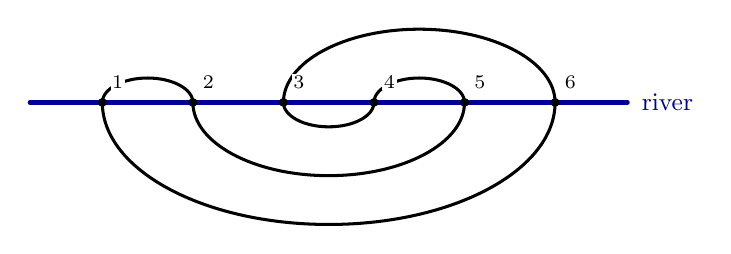
\begin{tikzpicture}[x=1.15cm,y=0.62cm,line cap=round]
  \draw[blue!60!black,line width=1.6pt] (0.2,0)--(6.8,0);
  \node[blue!60!black,anchor=west] at (6.85,0) {\small river};
  \begin{scope}[line width=1.1pt]\meanderroad\end{scope}
  \foreach \k in {1,...,6} {\fill (\k,0) circle[radius=1.6pt]; \node[fill=white,inner sep=0.6pt,font=\scriptsize] at (\k+0.17,0.42) {\k};}
\end{tikzpicture}}

% The series. Each paper cites the others as \cite{PaperA} etc.

\usetikzlibrary{intersections,calc}

\title{The subexponential factor of meander numbers\seriesline{Paper C.}}
\author{Carl Johan Ragnarsson}
\date{Draft of October 25, 2026}

\begin{document}
\maketitle

\begin{abstract}
A meander of order $n$ is a closed road that crosses a straight river $2n$ times without crossing
itself. Their number $M_n$ grows like $\mu^n$ with $\mu\approx12.26$, and the factor
$u_n=M_n/\mu^n$ that remains is conjectured to decay like a power $n^{-\alpha}$ with
$\alpha=(29+\sqrt{145})/12\approx3.4201$. This paper collects what can be proved about $u_n$. The
main result is that $\mu^n e^{-C\sqrt n}\le M_n\le\mu^{n+1}/(8n)$ for every $n$. The lower bound is
new; it removes a logarithmic factor from the previous one. Its proof cuts a meander into two balanced
halves and completes each half to a meander in a way that can be undone at small cost. Around these
bounds we prove the ratio limit $M_{n+1}/M_n\to\mu$ with a rate, the unique factorization of
meanders into prime meanders (those that are not obtained by gluing two smaller ones), the bound
$\sum_n u_n\le1/4$, a bound on the probability that a meander splits as such a product at a given
position, and comparisons with splittings that are nearly exact. For meanders whose crossing labels, a
height attached to each crossing, stay in $\{-1,0,1,2\}$, the growth rate and the exponent are found
exactly: the growth rate is a quartic irrational $10.4245\ldots$ and the exponent is $3.7758\ldots$,
given by the angle of a wedge in which a two-dimensional walk is confined. The generating function of
this bounded-label family is not D-finite: it satisfies no linear differential equation with polynomial
coefficients. Finally we state which
estimates would improve the bounds, show why some natural routes cannot, and list exact data. All code was written using
Claude (Opus 5.5) or Codex (Sol 5.1) with active review and guidance throughout.
\end{abstract}

%%%%%%%%%%%%%%%%%%%%%%%%%%%%%%%%%%%%%%%%%%%%%%%%%%%%%%%%%%%%%%%%%%%%%%%%
\section{Introduction}\label{sec:intro}
%%%%%%%%%%%%%%%%%%%%%%%%%%%%%%%%%%%%%%%%%%%%%%%%%%%%%%%%%%%%%%%%%%%%%%%%

\subsection{The factor \texorpdfstring{$u_n$}{u\_n}}

A \emph{meander of order $n$} is a closed road that crosses a straight river $2n$ times and never
crosses itself. Number the crossings $1,\ldots,2n$ from left to right along the river. Above the
river the road consists of $n$ \emph{arches}, each joining two crossings, and no two arches cross;
the same holds below the river. So a meander is a pair of noncrossing perfect matchings of
$\{1,\ldots,2n\}$, one drawn above and one below, whose union is a single closed curve.
Figure~\ref{fig:running} shows one of the eight meanders of order~$3$. The number $M_n$ of
meanders of order $n$ starts
\[ 1,\ 2,\ 8,\ 42,\ 262,\ 1828,\ 13820,\ 110954,\ \ldots \]
and is known exactly for every $n\le 32$ (OEIS A005315~\cite{OEIS} and~\cite{Jensen,JensenGit}). No formula is
known.

\begin{figure}[ht]
\centering
\meanderfigure
\caption{A meander of order $3$, the running example of the series. Above the river the road
joins crossings $1$--$2$, $3$--$6$ and $4$--$5$; below it joins $1$--$6$, $2$--$5$ and $3$--$4$.}
\label{fig:running}
\end{figure}

The growth rate $\mu=\lim_n M_n^{1/n}$ exists (Section~\ref{sec:growth}). Its value is about $12.26$,
and Paper~B of this series proves $12.2191\le\mu\le12.2970$~\cite{PaperB}. This paper is about
what is left once the exponential growth is removed,
\[ u_n \;=\; \frac{M_n}{\mu^n}. \]
Intuitively, $\mu^n$ accounts for the local freedom of the road, about $\mu$ choices for each new
pair of crossings, and $u_n$ is the remaining global correction. The physics prediction~\cite{DGG} is
\begin{equation}\label{eq:law}
u_n \;\approx\; A\,n^{-\alpha},\qquad \alpha=\alpha_*=\frac{29+\sqrt{145}}{12}\approx 3.4201,
\end{equation}
for a constant $A$. The prediction is not proved; numerical analysis of the exact counts
supports it~\cite{JG}. Paper~A explains where the number comes from~\cite{PaperA}, and Paper~D
studies the continuum model behind it~\cite{PaperD}. Throughout, $\alpha$ denotes the true exponent,
if it exists, and $\alpha_*$ the predicted number. We use the logarithmic form
\[ L(n) \;=\; n\log\mu-\log M_n \;=\; -\log u_n , \]
so that~\eqref{eq:law} reads $L(n)=\alpha\log n+O(1)$. We call $L(n)$ the \emph{loss} at order $n$.

\subsection{Main results}

Rigorous work on meanders has concentrated on the growth rate~\cite{AP,PaperB}. We are not aware
of earlier rigorous bounds on $u_n$ beyond $u_n\le1$, which follows from the existence of $\mu$;
our literature search was limited, and we claim no priority. The law~\eqref{eq:law} could fail in two
ways: $u_n$ could decay faster than every power, or it could be irregular. The results below address
both.

\begin{theorem}\label{thm:main}
There is a constant $C$ such that for every $n\ge1$
\[ \mu^n e^{-C\sqrt n} \;\le\; M_n \;\le\; \frac{\mu^{n+1}}{8n} . \]
\end{theorem}

So $u_n$ lies between $e^{-C\sqrt n}$ and $\mu/(8n)$. The upper bound on $u_n$ is already a power
law, with exponent $1$ in place of $3.42$; the lower bound $e^{-C\sqrt n}$ decays faster than every
power. In
logarithmic terms,
\[ \log n-\log(\mu/8) \;\le\; L(n) \;\le\; C\sqrt n, \]
while the prediction is $L(n)=3.4201\log n+O(1)$. The upper bound on $M_n$ comes from gluing two meanders of
order $n$ in at least $4n-1$ ways that can be told apart afterwards (Section~\ref{sec:upper}). The lower
bound is new. It improves the bound $L(n)\le C'\sqrt n\log n$ obtained earlier in this project, and it
comes from cutting a meander into two balanced pieces along a closed curve that meets the road and
the river about $\sqrt n$ times (Section~\ref{sec:lower}).

Around Theorem~\ref{thm:main} we prove or collect the following.
\begin{itemize}
\item \emph{Growth and ratios} (Section~\ref{sec:growth}). The ratio limit $M_{n+1}/M_n\to\mu$,
with the rate $|M_{n+1}/(\mu M_n)-1|\le C_{\mathrm r}\,n^{-1/4}\sqrt{\log n}$ for a constant
$C_{\mathrm r}$, improved to $O(n^{-1/4})$ by the lower bound of Theorem~\ref{thm:main}, and an exact
\emph{halving identity} that expresses $L(n)$ through the numbers
$D(m)=\log(M_{2m}/M_m^2)$, which measure how much more common a meander of order $2m$ is than a pair
of meanders of order $m$.
\item \emph{A subsequence result} (Section~\ref{sec:upper}). For every $\kappa<3/2$,
$\liminf_n n^\kappa u_n=0$. So if a power law holds, then $\alpha\ge3/2$.
\item \emph{Products and cuts} (Section~\ref{sec:products}). Two meanders can be glued side by side
into one, their \emph{product}; a \emph{cut} is a position where a meander comes apart as such a
product. Every meander factors uniquely into \emph{prime} meanders, those without a cut;
$\sum_n u_n\le 1/4$; the expected number of cuts is bounded; the probability of a cut at distance $s$
from the ends is at most $C_{\mathrm c}\,s^{-1/4}\sqrt{\log(s+1)}$; and \emph{near-cuts}, which
fail to be cuts in at most $K$ crossings, are at most $e^{O(K+1)}$ times more frequent than cuts.
\item \emph{An exactly solvable family} (Section~\ref{sec:band}). Each crossing of a meander carries
an integer \emph{label}, a signed count of the half turns the road makes on its way from the first crossing. For
meanders whose labels lie in $\{-1,0,1,2\}$, the count is $\Lambda^n n^{-\alpha_{\mathrm b}+o(1)}$ with
$\Lambda=10.4245\ldots$ and $\alpha_{\mathrm b}=3.7758\ldots$, both in closed form. Because
$\alpha_{\mathrm b}$ is irrational, the generating function of this family is not D-finite: it
satisfies no linear differential equation with polynomial coefficients.
\item \emph{Criteria} (Section~\ref{sec:improve}). Two conditional statements that would improve
the lower bound on $M_n$ to $L(n)=O(n^\tau)$ with $\tau<1/2$, a proof that gluing short meanders cannot supply
their hypotheses, a heuristic for what is true, and an exact reformulation of a weaker target.
\end{itemize}

\subsection{Status of the results}\label{sec:status}

Besides the lower bound of Theorem~\ref{thm:main}, the following are new as far as we know: the upper bound, the
subsequence result, the bound $\sum u_n\le1/4$, the cut bounds, the near-cut comparisons, the
results on bounded labels, including the corollary that the generating function of that family is not
D-finite (its main input is the exponent theorem), and the criteria of Section~\ref{sec:improve}. The
factorization into prime meanders is a close relative of known decompositions, and we claim no novelty for it.
% UNVERIFIED: the related decomposition into irreducible meanders in the physics literature was
% identified from a search summary; the paper itself was not read.

Most results were checked by a separate, independent reading of the written proof, which found no
gap. This includes both bounds of Theorem~\ref{thm:main}, the subsequence result, the ratio limit and
its rate (also in the improved form that uses Theorem~\ref{thm:main}), the factorization,
$\sum u_n\le1/4$, the near-cut comparisons, the growth rate and the exponent for bounded labels, the
irrationality of the exponent $\alpha_{\mathrm b}$, and the corollary on D-finiteness. The halving
identity and its corollary, the transcendence of $\alpha_{\mathrm b}$, the cut bound of
Proposition~\ref{prop:cutbound} and the criteria of Section~\ref{sec:improve} have complete written
proofs that have not been checked in this way.
Appendix~\ref{app:repo} gives the status of each result. Nothing in this paper has been reviewed
outside the project. Conjectures, heuristics and numerical statements are labeled as such. The exact
data in Appendix~\ref{app:data} use only the published counts $M_n$, $n\le32$.

%%%%%%%%%%%%%%%%%%%%%%%%%%%%%%%%%%%%%%%%%%%%%%%%%%%%%%%%%%%%%%%%%%%%%%%%
\section{Gluing and the growth rate}\label{sec:growth}
%%%%%%%%%%%%%%%%%%%%%%%%%%%%%%%%%%%%%%%%%%%%%%%%%%%%%%%%%%%%%%%%%%%%%%%%

\subsection{Terminology}

Let a meander of order $N$ have crossings $1,\ldots,2N$. The \emph{gap} $i$, for $0\le i\le 2N$, is
the stretch of river between crossings $i$ and $i+1$; gaps $0$ and $2N$ are the two ends. An arch
joining crossings $x<y$ \emph{passes over} gap $i$ if $x\le i<y$. An arch is \emph{exterior} if no
other arch on the same side encloses it, and \emph{short} if it joins two neighboring crossings.
The probability $\Pr_N$ and the expectation $\mathbb E_N$ refer to a meander of order $N$ chosen
uniformly at random.

\subsection{Supermultiplicativity and Fekete's lemma}

Two meanders can be glued into one. Let $G$ have order $a$ and $H$ order $b$. Place $H$ to the right
of $G$ on the same river. The last crossing $2a$ of $G$ is the right end of an exterior upper arch
$\{x,2a\}$, and the first crossing of $H$, now numbered $2a+1$, is the left end of an exterior upper
arch $\{2a+1,y\}$. Replace these two arches by $\{x,y\}$ and $\{2a,2a+1\}$. Nothing crosses, because
$\{x,y\}$ passes over everything between $x$ and $y$; and re-pairing one arch of each of two closed
curves joins them into one. Intuitively, both roads are cut open next to the boundary between them
and reconnected across it. The result $G\cdot H$ is a meander of order $a+b$, the \emph{product} of
$G$ and $H$. Given $a$, the pieces are recovered by undoing the re-pairing. Hence
\begin{equation}\label{eq:supermult}
M_{a+b}\;\ge\;M_aM_b\qquad\text{for all }a,b\ge1 .
\end{equation}
Section~\ref{sec:products} identifies exactly which meanders are products.

Inequality~\eqref{eq:supermult} says that $\log M_n$ is superadditive. Fekete's lemma~\cite{Fekete} then says
that $\log M_n/n$ converges to its supremum. The limit is finite because the upper and lower arch
systems are each counted by the Catalan number $\mathrm{Cat}_n=\binom{2n}{n}/(n+1)$, so
$M_n\le\mathrm{Cat}_n^2\le16^n$. Hence $\mu=\lim M_n^{1/n}$
exists, $\mu\le16$, and
\[ M_n\;\le\;\mu^n,\qquad\text{that is}\qquad u_n\le1 \quad\text{and}\quad L(n)\ge0 \qquad\text{for every } n. \]
In terms of $L$, inequality~\eqref{eq:supermult} says that $L$ is \emph{subadditive},
\begin{equation}\label{eq:subadd}
L(a+b)\;\le\;L(a)+L(b),
\end{equation}
and the existence of $\mu$ says $L(n)/n\to0$. These three facts about $L$ (it is nonnegative,
subadditive, and $o(n)$) are used repeatedly.

\subsection{The ratio limit}

\begin{theorem}[ratio limit]\label{thm:ratio}
$M_{n+1}/M_n\to\mu$. In particular the largest ratio $R_\star=\sup_n M_{n+1}/M_n$ is finite.
\end{theorem}

The proof rests on an exact identity. A \emph{wiggle} is a short upper arch followed by a short lower
arch, on three consecutive crossings $i,i+1,i+2$. Any crossing $x$ of a meander of order $n$ can be
replaced by three consecutive crossings that form a wiggle, with the old arches at $x$ reattached to
the outer two. This keeps the road one loop and gives a meander of order $n+1$ with a marked wiggle;
collapsing the marked wiggle undoes it. So marked crossings of order-$n$ meanders correspond exactly to
marked wiggles of order-$(n+1)$ meanders, and with $Z$ the number of wiggles,
\[ M_{n+1}\,\mathbb E_{n+1}[Z] \;=\; 2n\,M_n . \]
A further counting argument with these insertions shows that $Z/n$ concentrates at $2/\mu$ with exponentially small error probabilities, in
both directions. The identity then gives
$M_{n+1}/M_n=2n/\mathbb E_{n+1}[Z]\to\mu$. Since $Z\le n+1$, it also gives $M_{n+1}\ge M_n$: the counts never decrease.

The ratio limit has a rate. Its proof combines a lower bound on $M_n$ with two inequalities that
hold for every $n\ge3$, with a constant $C_0$:
\begin{equation}\label{eq:ratioinput}
\frac{M_{n+1}}{\mu M_n}\;\ge\;1-C_0\sqrt{\frac{L(n)+\log n}{n}},\qquad
\frac{\mu M_n}{M_{n+1}}\;\ge\;1-C_0\sqrt{\frac{L(n+1)+\log n}{n}} .
\end{equation}
The first bounds the ratio from below and the second bounds it from above. Both come from a further
structural decomposition of meanders that we do not describe here~\cite{Repo}. A lower bound on
$M_n$ is an upper bound on the loss $L$, and it makes both right sides close to $1$.

\begin{theorem}[rate in the ratio limit]\label{thm:rate}
There is a constant $C_{\mathrm r}$ such that for every $n\ge2$
\[ \Big|\frac{M_{n+1}}{\mu M_n}-1\Big| \;\le\; C_{\mathrm r}\, n^{-1/4}\sqrt{\log n} . \]
Consequently $|\log(u_{n+k}/u_n)|\le C_{\mathrm r}'\,k\,n^{-1/4}\sqrt{\log n}$ for $0\le k\le n$.
\end{theorem}

The constants are large: with the constants of the proof the bound says something only for $n$
beyond about $10^{14}$. The proof inserts the earlier lower bound $L(n)\le C'\sqrt n\log n$
into~\eqref{eq:ratioinput}. With Theorem~\ref{thm:main} in its place the factor $\sqrt{\log n}$
disappears, by the following short argument, which we give in full.

\begin{remark}
There is a constant $C_{\mathrm r}''$ such that $|M_{n+1}/(\mu M_n)-1|\le C_{\mathrm r}''\,n^{-1/4}$ for every
$n\ge2$. Indeed, by Theorem~\ref{thm:main}, $L(n)\le C\sqrt n$ and $L(n+1)\le2C\sqrt n$, so both right
sides of~\eqref{eq:ratioinput} are at least $1-\epsilon_n$ with $\epsilon_n=O(n^{-1/4})$; when
$\epsilon_n\le1/2$ the second inequality gives $M_{n+1}/(\mu M_n)\le1/(1-\epsilon_n)\le1+2\epsilon_n$, and
the finitely many other $n$ are covered by $M_{n+1}/M_n\le R_\star$ after enlarging the constant.
Summing the logarithms as in Theorem~\ref{thm:rate} gives $|\log(u_{n+k}/u_n)|=O(k\,n^{-1/4})$ for
$0\le k\le n$, and the proof of Proposition~\ref{prop:cutbound} below, run with this rate, improves
the cut bound to $O(s^{-1/4})$. The inequalities~\eqref{eq:ratioinput} cannot give more than
$n^{-1/4}$: sequences of the same form as the decomposition behind them, with loss of order $\sqrt n$, can
have ratios that differ from $\mu$ by a multiple of $n^{-1/4}$ infinitely often~\cite{Repo}.
\end{remark}

Theorem~\ref{thm:rate} says that $u_n$ is \emph{locally smooth}: it changes by a bounded factor over
windows of length about $n^{1/4}/\sqrt{\log n}$, and by the remark over windows of length about
$n^{1/4}$. It does not say that $u_n$ is decreasing: the
statement $M_{n+1}\le\mu M_n$ for all $n$ is open. It holds for every $n\le31$, since the ratios
$M_{n+1}/M_n$ increase in that range and $M_{32}/M_{31}=11.023$ is below the lower bound
$12.2191$ for $\mu$.

\subsection{The halving identity}

The \emph{doubling defect} is
\[ D(m)\;=\;\log\frac{M_{2m}}{M_m^2}\;=\;2L(m)-L(2m) . \]
By~\eqref{eq:supermult}, $D(m)\ge0$. Section~\ref{sec:products} shows that $e^{-D(m)}$ is exactly
the probability that a random meander of order $2m$ is a product of two meanders of order $m$.

\begin{proposition}[halving identity]\label{prop:halving}
For every $n\ge1$,
\[ L(n)\;=\;\sum_{j\ge0}2^{-(j+1)}D(2^jn). \]
\end{proposition}

\begin{proof}
Since $D(m)=2L(m)-L(2m)$, the partial sums telescope:
$\sum_{j=0}^{J-1}2^{-(j+1)}D(2^jn)=L(n)-2^{-J}L(2^Jn)$. The last term is
$n\cdot L(2^Jn)/(2^Jn)$, which tends to $0$ because $L(k)/k\to0$.
\end{proof}

The right side involves only the counts, not $\mu$. Intuitively, the identity starts from a huge
meander, halves it again and again down to order $n$, and adds up what each halving costs. It turns statements about $u_n$ into
statements about the single sequence $D(m)$.

\begin{corollary}\label{cor:halving}
For a constant $\alpha$:
\begin{enumerate}
\item $L(n)=\alpha\log n+O(1)$ for all $n$ if and only if $D(m)=\alpha\log m+O(1)$;
\item $L(n)=\alpha\log n+o(\log n)$ if and only if $D(m)=\alpha\log m+o(\log m)$;
\item $L(n)\le\chi\log n+O(1)$ for some $\chi$ if and only if $D(m)\le\chi'\log m+O(1)$ for some $\chi'$.
\end{enumerate}
\end{corollary}

\begin{proof}
In each part, one direction follows from $D(m)=2L(m)-L(2m)$ and the other from the identity. For
example, in part 1, if $|D(m)-\alpha\log m|\le c$ for all $m$, then
\[ L(n)=\sum_{j\ge0}2^{-(j+1)}\big(\alpha\log n+\alpha j\log 2+O(c)\big)
 =\alpha\log n+\alpha\log2+O(c), \]
using $\sum_j 2^{-(j+1)}=1$ and $\sum_j j\,2^{-(j+1)}=1$. Part 3 is the same computation with inequalities, using $L\ge0$, and part 2 uses that $\epsilon\log(2^jn)\le\epsilon(\log n+j\log2)$.
\end{proof}

So the power law~\eqref{eq:law} is equivalent to $D(m)=\alpha\log m+O(1)$: the probability that a
meander of order $2m$ splits into two meanders of order $m$ should decay like $m^{-\alpha}$. If $u_n\sim An^{-\alpha}$,
then $D(2m)-D(m)$ tends to $\alpha\log 2\approx2.371$; if in addition the correction is smooth, for example
$u_n=An^{-\alpha}(1+O(1/n))$, then $m\,(D(m+1)-D(m))$ tends to $\alpha$.
Table~\ref{tab:D} in Appendix~\ref{app:data} lists exact values. Along the computed range $D$ is
increasing and concave, and both of these quantities increase, reaching $3.13$ at $m=15$ and $2.19$
at $m=8$. Theorem~\ref{thm:main} gives $D(m)\le 2L(m)\le 2C\sqrt m$.

%%%%%%%%%%%%%%%%%%%%%%%%%%%%%%%%%%%%%%%%%%%%%%%%%%%%%%%%%%%%%%%%%%%%%%%%
\section{The upper bound}\label{sec:upper}
%%%%%%%%%%%%%%%%%%%%%%%%%%%%%%%%%%%%%%%%%%%%%%%%%%%%%%%%%%%%%%%%%%%%%%%%

The bound $M_n\le\mu^n$ uses one way of gluing two meanders. The bound $M_n\le\mu^{n+1}/(8n)$ uses
many: if two meanders of order $n$ can be glued in at least $4n-1$ ways that can be told apart afterwards,
then meanders of order about $2n$ are about $n$ times as many as pairs of meanders of order $n$,
and that forces a factor $1/n$. The device of joining two objects of equal size in many
recognizable ways goes back to work of Madras on lattice trees~\cite{Madras}.
% UNVERIFIED: the Madras attribution rests on the abstract of his J. Stat. Phys. 78 (1995) paper only;
% the full text was not read.

\subsection{Capped blocks}

Let $\Gamma$ be a meander of order $N$. A \emph{capped block} of $\Gamma$ is a lower arch
$\{\ell,\ell'\}$ with $\ell'\ge\ell+3$ such that every upper arch with an end in
$\{\ell+2,\ldots,\ell'\}$ has both ends there. Its \emph{size} is $\ell'-\ell+1$, the number of
crossings from $\ell$ to $\ell'$. Intuitively, a capped block is a small meander hanging under one
lower arch, attached to the rest of the road only through the two crossings $\ell$ and $\ell+1$. The
size is always even, $2b+2$ with $b\ge1$, and the road inside the block is a single path through all
its crossings. Two lower arches are nested or disjoint, so two capped blocks are nested or disjoint.
Two capped blocks with more than $N$ crossings each, out of $2N$, must overlap and are therefore
nested; so a meander has at most one capped block of each size larger than~$N$.

\emph{Insertion.} The upper arches of a meander cut the half-plane above the river into
\emph{regions}. Let $G$ be a meander of order $a$, let $i$ be one of its $2a+1$ gaps, and let
$\{p,q\}$ be an upper arch on the boundary of the region that lies directly above gap $i$. Let
$H$ be a meander of order $b$. Put $2b+2$ new crossings into gap $i$: the crossings of $H$, with one
extra crossing on each side, $\ell$ on the left and $\ell'$ on the right, joined by a new lower arch
that caps them. Remove $\{p,q\}$ and the upper arch $\{\ell+1,y_1\}$ at the first crossing of $H$.
Add the upper arch $\{y_1,\ell'\}$, and join $\ell$ and $\ell+1$ to $p$ and $q$ by two upper arches, in
the one of the two possible pairings that crosses nothing. Because $\{p,q\}$ lies on the boundary of
the region containing the gap, no other arch is crossed. The road becomes one loop, and the new lower arch spans a capped block
of size $2b+2$. Extraction reverses this. Intuitively, $H$ is opened at its first crossing and spliced
into the road of $G$ at the arch $\{p,q\}$.

\begin{theorem}[insertion bijection]\label{thm:insertion}
For $a,b\ge1$ and $N=a+b+1$, insertion is a bijection from the quadruples $(G,i,\{p,q\},H)$ onto the
pairs (meander $\Gamma$ of order $N$, capped block of $\Gamma$ of size $2b+2$).
\end{theorem}

Write $T(G)$ for the number of pairs $(i,\{p,q\})$ available in $G$, and $T_a=\sum_G T(G)$, the sum over
meanders $G$ of order $a$. The theorem says that the meanders of order $N$, counted with their number of capped
blocks of size $2b+2$, total $T_aM_b$. For $a\le b$ the block has $2b+2\ge N+1$ crossings and is
unique, which gives
\begin{equation}\label{eq:insertion}
M_{a+b+1}\;\ge\;T_aM_b\qquad(1\le a\le b).
\end{equation}

\begin{lemma}\label{lem:faces}
For every meander $G$ of order $a$, $T(G)\ge4a-1$. Hence $T_a\ge(4a-1)M_a$.
\end{lemma}

\begin{proof}
The $a$ upper arches cut the upper half-plane into $a+1$ regions; the pairs $(i,\{p,q\})$ counted by
$T(G)$ are, region by region, a gap in it times an arch on its boundary. A bounded region lies directly
under one arch with $k$ arches directly below it; it has $k+1$ arches on its boundary and contains
$k+1$ gaps. The unbounded region has $c$ exterior arches on its boundary and contains $c+1$ gaps. So
$T(G)=\sum_F c_F^2+c_\infty$, where $c_F\ge1$ is the number of arches on the boundary of region $F$
and $c_\infty=c$. Every arch bounds two regions, so $\sum_Fc_F=2a$. For positive integers
$c^2\ge3c-2$, so $\sum_Fc_F^2\ge 6a-2(a+1)=4a-2$, and $c_\infty\ge1$.
\end{proof}

\subsection{The doubling argument}

\begin{proof}[Proof of the upper bound in Theorem~\ref{thm:main}]
Put $g(n)=8n\,M_n$. By~\eqref{eq:insertion} with $a=b=n$ and Lemma~\ref{lem:faces},
\[ g(2n+1)=8(2n+1)M_{2n+1}\;\ge\;8(2n+1)(4n-1)M_n^2\;\ge\;64n^2M_n^2=g(n)^2 , \]
because $8(2n+1)(4n-1)=64n^2+16n-8\ge64n^2$. Since $(2n+1)+1=2(n+1)$, the numbers
$f(n)=\log g(n)/(n+1)$ satisfy $f(2n+1)\ge f(n)$. Let $n^{(0)}=n$ and $n^{(k+1)}=2n^{(k)}+1$, so
$n^{(k)}+1=2^k(n+1)$. Then
\[ f(n)\;\le\;f(n^{(k)})\;=\;\frac{\log(8n^{(k)})}{n^{(k)}+1}+\frac{n^{(k)}}{n^{(k)}+1}\cdot\frac{\log M_{n^{(k)}}}{n^{(k)}}
\;\longrightarrow\;\log\mu \qquad(k\to\infty). \]
So $\log g(n)\le(n+1)\log\mu$, that is $8nM_n\le\mu^{n+1}$.
\end{proof}

Every $n$ starts its own chain $n,2n+1,4n+3,\ldots$, so the bound holds at every $n$ and needs no
regularity of $u_n$. The constant $8$ cannot be improved by this argument. On the exact data,
$(8nM_n)^{1/(n+1)}\le9.07$ for $n\le32$, well below $\mu$, so the bound is far from tight there. In
terms of the loss it says $L(n)\ge\log n-\log(\mu/8)$. Combined with $M_{2m+1}\le R_\star M_{2m}$, inequality~\eqref{eq:insertion} with $a=b=m$ also gives
$D(m)\ge\log(4m-1)-\log R_\star$; under the power law this says again that $\alpha\ge1$.

\subsection{The exponent \texorpdfstring{$3/2$}{3/2} along a subsequence}

Insertion can be repeated. Let $H_1$ and $H_2$ be meanders of orders $b_1$ and $b_2$, and let
$\mathrm{wrap}(H_2)$ be the meander of order $b_2+1$ in which $H_2$ hangs as a capped block under one
new lower arch. Inserting the product $H_1\cdot\mathrm{wrap}(H_2)$ into $G$ gives a map that is again
one-to-one with a recognizable image: the inserted block is the smallest capped block with more than
$N$ crossings. The result is a three-piece inequality.

\begin{theorem}[three-piece insertion]\label{thm:threepiece}
For $N\ge5$,
\[ M_N\;\ge\;\sum T_a\,M_{b_1}M_{b_2}, \]
the sum over positive integers with $a+b_1+b_2=N-2$, $2a\le N-1$, $2b_1\le N$ and $2b_2+2\le N$.
\end{theorem}

\begin{theorem}\label{thm:threehalves}
For every $\kappa<3/2$, $\liminf_{n\to\infty}n^\kappa u_n=0$. Equivalently,
$\limsup_n L(n)/\log n\ge3/2$.
\end{theorem}

\begin{proof}
Suppose $u_n\ge c_\kappa n^{-\kappa}$ for all large $n$, with $\kappa<3/2$. If $\kappa<1$ this already
contradicts $u_n\le\mu/(8n)$, so let $1\le\kappa<3/2$. In
Theorem~\ref{thm:threepiece} keep the triples with $a$ and $b_1$ in $[N/4,3N/8]$. There are at least
$N^2/256$ of them for large $N$, each has $T_a\ge(4a-1)M_a\ge (N/2)M_a$, and all three sizes are at
least $N/4-2$. Inserting the assumed lower bound for $M_a$, $M_{b_1}$, $M_{b_2}$ gives
$u_N\ge c_\kappa'N^{-(3\kappa-3)}$ for large $N$. Since $3/2-(3\kappa-3)=3(3/2-\kappa)$, the distance to
$3/2$ triples at each step, so after finitely many steps the exponent is below $1$. That contradicts
$u_n\le\mu/(8n)$.
\end{proof}

So if a power law $u_n=n^{-\alpha+o(1)}$ holds, then $\alpha\ge3/2$. Without that assumption,
Theorem~\ref{thm:threehalves} says only that no lower bound $c_\kappa n^{-\kappa}$ with $\kappa<3/2$ holds
for all large $n$; it does not give $u_n=O(n^{-3/2})$. Heuristically, $3/2$ is the limit of
the method: Theorem~\ref{thm:threepiece} is nearly an equality when $u_n$ is of order $n^{-3/2}$,
which is the behavior of tree-like families built only by insertion and products. Going further needs
an input that separates meanders from such families. One candidate is that a positive fraction of
meanders of order $n$ has no capped block with more than $n$ crossings; with it the same argument
gives $\kappa<2$. In the exact data this fraction is $0.5$ at $n=2$ and $3$ and about $0.85$ at
$n=24$ and $25$, but it is not proved to stay positive.

%%%%%%%%%%%%%%%%%%%%%%%%%%%%%%%%%%%%%%%%%%%%%%%%%%%%%%%%%%%%%%%%%%%%%%%%
\section{The lower bound}\label{sec:lower}
%%%%%%%%%%%%%%%%%%%%%%%%%%%%%%%%%%%%%%%%%%%%%%%%%%%%%%%%%%%%%%%%%%%%%%%%

The lower bound needs the opposite of~\eqref{eq:supermult}: a large meander must not be much more
common than a pair of smaller ones. The proof has four steps. A closed curve, the
\emph{separator}, cuts every meander into two pieces of comparable size and meets the road and the
river only about $\sqrt N$ times (Section~\ref{sec:separator}). Each piece is completed to a meander
in a way that can be undone with little extra information (Section~\ref{sec:disc}). This gives a
reverse inequality $M_N\le e^{B\sqrt N}M_aM_b$ with $a,b$ comparable to $N/2$
(Section~\ref{sec:reverse}). Repeated splitting, together with subadditivity, turns it into
$L(n)\le C\sqrt n$ (Section~\ref{sec:descent}).

The $\sqrt n$ has a plain source. The cost of the cut is exponential in the number of times the
separator meets the road and the river. Some planar graphs really need about $\sqrt N$ such meetings
to be cut into two pieces of comparable size; a square grid of side $\sqrt N$ is the standard
example. Since the argument is applied to every meander, it must pay for the worst case. Whether a
typical meander can be cut more cheaply is not known; Section~\ref{sec:improve} states what a cheaper
cut would give.

\subsection{A balanced separator}\label{sec:separator}

Close the river through a point at infinity, so that river and road become two closed curves on the
sphere that cross at $2N$ points. Together they form a \emph{planar map}, a graph drawn on the
sphere, with $2N$ vertices, each of degree four. A \emph{separator} is a closed curve on the sphere
that avoids the $2N$ crossings and crosses the river and the road transversally. The points where it
crosses them are called \emph{ports}. It splits the sphere into two disks.

\begin{proposition}[single balanced separator]\label{prop:noose}
For every sufficiently large $N$, every meander of order $N$ has a separator with at most
$4\sqrt{27N}$ ports such that each of its two disks contains between $N/2$ and $3N/2$ of the $2N$
crossings.
\end{proposition}

The proof applies published theorems rather than proving a new one. Subdivide every edge
of the map once, which gives a simple connected plane graph with $6N$ vertices, none of degree one.
Its \emph{branchwidth}, a standard measure of how cheaply a graph can be cut up, is at most
$\sqrt{4.5\cdot 6N}=\sqrt{27N}$ by a theorem of Fomin and Thilikos~\cite{FominThilikos}, which bounds
the branchwidth of a planar graph with $v$ vertices by $\sqrt{4.5v}$. By Seymour and Thomas~\cite{ST}
and Gu and Tamaki~\cite{GuTamaki}, in the form given by Dorn, Penninkx, Bodlaender and
Fomin~\cite{DPBF}, such a graph has a \emph{sphere-cut decomposition} of the same width. This is a tree whose leaves are the edges of the graph and in which
every tree edge corresponds to a closed curve on the sphere that meets the graph in at most
$\sqrt{27N}$ vertices and separates the graph edges on the two sides of the tree edge. Give each
original crossing weight one, placed on a leaf at that crossing; a weighted centroid of the tree has
an incident edge whose curve splits the weight between $2N/3$ and $4N/3$. Finally push the curve off
each vertex it passes through; this creates at most four ports per vertex. Balanced separators of
order $\sqrt N$ are classical for planar graphs~\cite{LT,Miller}; what matters here is that this one
is a single closed curve, so that each side is one disk and all loose ends of a side lie on one
circle.

\subsection{Disk completion with a protective cycle}\label{sec:disc}

Cut the sphere along the separator. Each side is a \emph{disk patch}: some $v$ crossings, pieces of
river and road inside, and $w$ ports on the boundary circle. The river and the road each have a
positive even number of ports, since each closed curve visits both sides. The task is to turn a patch
into a meander from which the patch can be read off again.

\begin{proposition}[disk completion]\label{prop:disc}
There is an absolute constant $c_\Omega$ with the following property. Every disk patch with $v$ crossings
and $w$ ports can be completed to a meander with at most $v+8w$ crossings, in such a way that the patch,
with the cyclic order of its ports, is recovered from the completed meander, a marked crossing of it,
and a \emph{record} taking at most $e^{c_\Omega w}$ possible values.
\end{proposition}

Intuitively, the completed meander does not show where the patch sits inside it; the marked crossing
and the record say where to find it. The construction has two parts, a cycle and caps, and the
recovery uses the cycle; Figure~\ref{fig:separator} sketches it.

\emph{The protective cycle.} Just outside the boundary, draw a closed curve $\Omega$ around the patch that
crosses each port strand once. Call the river and the road the two \emph{colors}; a crossing always
joins strands of different colors. So along a stretch of $\Omega$ that crosses road strands, $\Omega$ is
made of river, and along a stretch that crosses river strands, $\Omega$ is made of road. Where the color
of the ports changes,
$\Omega$ switches color: its river part and its road part cross at one new crossing, both continue
outward past it, and $\Omega$ turns there from one to the other. So $\Omega$ is a cycle of the new map
with at most $2w$ vertices: at a port it goes straight through, and at a switch it turns.

\emph{Caps.} Outside $\Omega$, every piece of river and every piece of road is an arc with two loose ends,
because no closed curve can lie entirely in one patch. For each color, join the loose ends outside
by a noncrossing family of arcs, the \emph{caps}, nested at most two deep and chosen so that each
color closes into a single curve. This can always be done by scanning the ends once around the circle
and merging pieces one at a time. There are at most $3w$ loose ends: one for each port, and two for each switch.
Each crossing between caps of different colors can be charged to an end of one color lying under a
cap of the other color, and since caps are nested at most two deep, each end carries at most two
charges. So the caps add at most $6w$ crossings. Together with the at most $2w$ vertices of $\Omega$, the completion has at most $v+8w$
crossings.

\emph{Recovery.} Mark a vertex of $\Omega$ and record, step by step, how $\Omega$ continues: at each vertex of a
map of degree four there are at most three ways to continue without going back, so the record has at most
$3^{2w}$ possibilities. One more bit says which side of $\Omega$ holds the patch. The record recovers $\Omega$.
At a vertex where $\Omega$ goes straight, one strand enters the inside: that is a port. At a switch no
strand enters. Deleting $\Omega$ and everything outside recovers the patch and the cyclic order of its
ports.

The point of the protective cycle is that it is \emph{recognizable}. Without it, an earlier
completion had to record which edges the cut had crossed, which takes $N^{O(w)}$ possible records
instead of $e^{c_\Omega w}$. With $w$ of order $\sqrt N$, that is the difference between
$e^{O(\sqrt N\log N)}$ and $e^{O(\sqrt N)}$.

\begin{figure}[t]
\centering
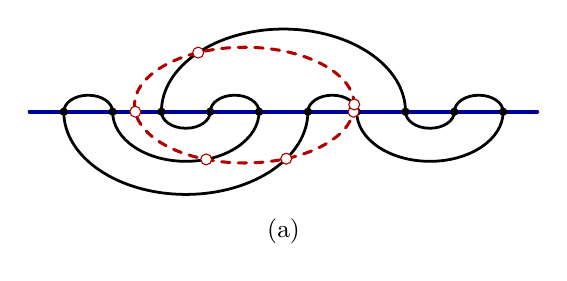
\begin{tikzpicture}[x=0.62cm,y=0.42cm,line cap=round]
  \draw[blue!60!black,line width=1.4pt,name path=river] (0.3,0)--(10.7,0);
  \begin{scope}[line width=1pt]
    \draw[name path global=a1] (1,0) arc[start angle=180,end angle=0,radius=0.5];
    \draw[name path global=a2] (3,0) arc[start angle=180,end angle=0,radius=2.5];
    \draw[name path global=a3] (4,0) arc[start angle=180,end angle=0,radius=0.5];
    \draw[name path global=a4] (6,0) arc[start angle=180,end angle=0,radius=0.5];
    \draw[name path global=a5] (9,0) arc[start angle=180,end angle=0,radius=0.5];
    \draw[name path global=b1] (1,0) arc[start angle=180,end angle=360,radius=2.5];
    \draw[name path global=b2] (2,0) arc[start angle=180,end angle=360,radius=1.5];
    \draw[name path global=b3] (3,0) arc[start angle=180,end angle=360,radius=0.5];
    \draw[name path global=b4] (7,0) arc[start angle=180,end angle=360,radius=1.5];
    \draw[name path global=b5] (8,0) arc[start angle=180,end angle=360,radius=0.5];
  \end{scope}
  \foreach \k in {1,...,10} \fill (\k,0) circle[radius=1.5pt];
  \draw[red!70!black,line width=1.1pt,dashed,name path=sep] (4.7,0.2) ellipse[x radius=2.25,y radius=1.75];
  \foreach \p in {river,a1,a2,a3,a4,a5,b1,b2,b3,b4,b5}{
    \path[name intersections={of=sep and \p,name=I,total=\t}] \pgfextra{\xdef\tot{\t}};
    \ifnum\tot>0
      \foreach \s in {1,...,\tot}{\node[draw=red!70!black,fill=white,circle,inner sep=1.4pt] at (I-\s) {};}
    \fi
  }
  \node[font=\small] at (5.5,-3.6) {(a)};
\end{tikzpicture}
\hspace{0.6cm}
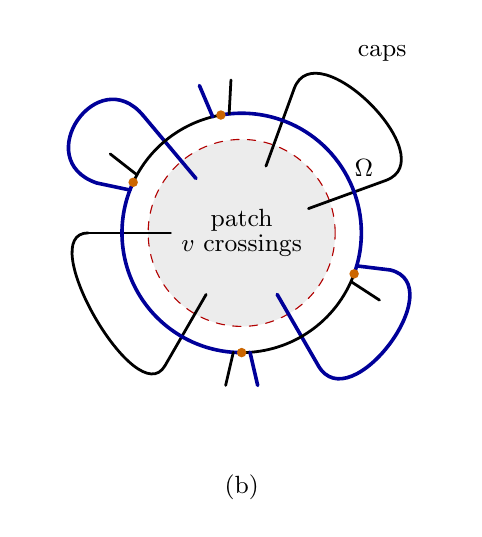
\begin{tikzpicture}[scale=0.95,line cap=round]
  \fill[gray!15] (0,0) circle[radius=1.25];
  \node[font=\small,align=center] at (0,0) {patch\\[-2pt]$v$ crossings};
  \draw[red!70!black,dashed] (0,0) circle[radius=1.25];
  % ports: road at 20,70,180,240; river at 130,300
  \foreach \a in {20,70,180,240} \draw[line width=1pt] (\a:0.95)--(\a:2.05);
  \foreach \a in {130,300} \draw[blue!60!black,line width=1.3pt] (\a:0.95)--(\a:2.05);
  % protective cycle: river-colored over road ports, road-colored over river ports
  \draw[blue!60!black,line width=1.3pt] (-20:1.6) arc[start angle=-20,end angle=100,radius=1.6];
  \draw[line width=1pt] (100:1.6) arc[start angle=100,end angle=155,radius=1.6];
  \draw[blue!60!black,line width=1.3pt] (155:1.6) arc[start angle=155,end angle=270,radius=1.6];
  \draw[line width=1pt] (270:1.6) arc[start angle=270,end angle=340,radius=1.6];
  % switch stubs, one of each color
  \foreach \a in {100,155,270,340}{
    \draw[line width=1pt] (\a-4:1.6)--(\a-6:2.05);
    \draw[blue!60!black,line width=1.3pt] (\a+4:1.6)--(\a+6:2.05);
    \fill[orange!80!black] (\a:1.6) circle[radius=1.8pt];
  }
  % schematic caps outside
  \draw[line width=1pt] (20:2.05) .. controls (20:2.9) and (70:2.9) .. (70:2.05);
  \draw[blue!60!black,line width=1.3pt] (130:2.05) .. controls (130:3.0) and (161:3.0) .. (161:2.05);
  \draw[line width=1pt] (180:2.05) .. controls (180:2.8) and (240:2.8) .. (240:2.05);
  \draw[blue!60!black,line width=1.3pt] (300:2.05) .. controls (300:2.9) and (346:2.9) .. (346:2.05);
  \node[font=\small] at (52:3.05) {caps};
  \node[font=\small] at (28:1.85) {$\Omega$};
  \node[font=\small] at (0,-3.4) {(b)};
\end{tikzpicture}
\caption{(a) The meander of Figure~\ref{fig:cut} with a separator (dashed). Its ports, the
points where it crosses the river or the road, are circled. (b) Completion of one side, schematically:
the patch inside the separator, the protective cycle $\Omega$ just outside it (river-colored where it
crosses road strands, road-colored where it crosses river strands, switching color at the dots), and
caps outside that close each color into one curve. The caps shown are only indicative.}
\label{fig:separator}
\end{figure}

\subsection{The reverse inequality}\label{sec:reverse}

\begin{proposition}[reverse inequality]\label{prop:reverse}
There is a constant $B$ such that for every sufficiently large $N$
\[ M_N\;\le\;e^{B\sqrt N}\max M_aM_b, \]
the maximum over integers $a,b$ with $N\le a+b\le N+8W$ and $N/10\le a,b\le 9N/10$, where
$W=\lceil4\sqrt{27N}\rceil$.
\end{proposition}

\begin{proof}[Key idea]
Choose, for each meander of order $N$, one separator as in Proposition~\ref{prop:noose}, with
$w\le W$ ports, and complete both sides as in Proposition~\ref{prop:disc}. The sides have $v_1+v_2=2N$
crossings with $N/2\le v_i\le3N/2$, and the completed meanders have orders $a$, $b$ with
$v_i/2\le a,b\le v_i/2+4w$. The original meander is recovered from the two completed meanders with
one marked crossing each, their two records, and the way the two boundary circles are glued, which
is an orientation and a rotation, at most $2w$ choices. The marks, the sizes, and the choice of which
crossing of the glued map is crossing $1$ of the original meander, and in which direction the river
runs, cost only a fixed polynomial in $N$. So the number of meanders of order $N$ is at
most a polynomial in $N$ times $e^{2c_\Omega W}$ times $\max M_aM_b$, and the polynomial is absorbed into
$e^{B\sqrt N}$. The ranges of $a$, $b$ follow from those of $v_i$ for large $N$.
\end{proof}

No ratio bound is used: the sizes $a$ and $b$ are allowed to exceed $N$ in total by $O(\sqrt N)$, and
that excess is handled in the next step by $\mu\le16$.

\subsection{The descending chain}\label{sec:descent}

\begin{proof}[Proof of the lower bound in Theorem~\ref{thm:main}]
By Proposition~\ref{prop:reverse}, for every large $N$ there are $a,b\in[N/10,9N/10]$ with
\[ L(a)+L(b)\;\le\;L(N)+(a+b-N)\log\mu+B\sqrt N\;\le\;L(N)+B_1\sqrt N , \]
using $a+b-N\le8W$ and $\mu\le16$. Divide by $a+b\ge N$ and use $L(N)\ge0$: one of the two, call it
$k$ and call it a \emph{child} of $N$, satisfies
\begin{equation}\label{eq:child}
\frac{L(k)}{k}\;\le\;\frac{L(N)}{N}+\frac{B_1}{\sqrt N}.
\end{equation}
Intuitively, passing to a child increases the loss per crossing, $L(k)/k$, only slightly. Fix a large target $n$ and start
from a huge $N_0$. Pass repeatedly to a child, and stop at the first size $k\le n$; then
$n/10<k\le n$. Each step
shrinks the size by a factor between $1/10$ and $9/10$, so, read backward from the last one, the
sizes grow at least geometrically and the added terms $B_1/\sqrt{\text{size}}$ sum to at most a
constant times $1/\sqrt n$. Choosing $N_0$ so large that $L(N_0)/N_0\le1/\sqrt n$ gives a $k$ in
$(n/10,n]$ with $L(k)\le B_2\sqrt n$, for every large $n$.

Now take any $n$. Split off such a size $k_1\in(n/10,n]$, then such a size $k_2$ for the remainder
$n-k_1\le9n/10$, and so on. By subadditivity~\eqref{eq:subadd}, $L(n)$ is at most
$L(k_1)+L(k_2)+\cdots$ plus a bounded term for the last small remainder. Each $L(k_i)$ is at most
$B_2$ times the square root of a geometrically decreasing size, so the sum is at most a constant
times $\sqrt n$. This gives
$L(n)\le C\sqrt n$ for large $n$, and enlarging $C$ covers small $n$.
\end{proof}

The same descent turns a reverse inequality $M_N\le e^{O(N^\tau)}\max M_aM_b$, for a fixed
$0<\tau<1$, into $L(n)=O(n^\tau)$, provided that the maximum runs over sizes $a,b$ between two fixed
fractions of $N$ with $a+b-N=O(N^\tau)$. The excess $a+b-N$ costs $(a+b-N)\log\mu$ in the first
display of the proof, and under these conditions the geometric sums still converge. Both conditions
are needed: with the excess $8W$ of Proposition~\ref{prop:reverse}, which is of order $\sqrt N$, the
descent gives only $L(n)=O(\sqrt n)$, however small the factor $e^{O(N^\tau)}$ is. With the earlier
completion the loss was
of order $\sqrt N\log N$, which gave the previous bound. The argument also extends, with the same
square root, to systems of several closed roads weighted by a parameter for each road; we do not use
this here.

%%%%%%%%%%%%%%%%%%%%%%%%%%%%%%%%%%%%%%%%%%%%%%%%%%%%%%%%%%%%%%%%%%%%%%%%
\section{Products, primes and cuts}\label{sec:products}
%%%%%%%%%%%%%%%%%%%%%%%%%%%%%%%%%%%%%%%%%%%%%%%%%%%%%%%%%%%%%%%%%%%%%%%%

\subsection{Cuts}

\begin{definition}
A meander of order $N$ has a \emph{cut} at $m$, for $1\le m\le N-1$, if no lower arch passes over
gap $2m$, the crossings $2m$ and $2m+1$ are joined by a short upper arch, and exactly one other upper
arch passes over gap $2m$.
\end{definition}

Intuitively, a cut is a thin neck: the road passes from the left part of the river to the right part
exactly twice, once along the short arch and once along the arch over it. Figure~\ref{fig:cut} shows
an example. The product of Section~\ref{sec:growth} creates exactly such a neck.

\begin{theorem}[products and cuts]\label{thm:cuts}
The product $(G,H)\mapsto G\cdot H$ of Section~\ref{sec:growth} is a bijection from pairs of meanders
of orders $m$ and $N-m$ onto meanders of order $N$ with a cut at $m$. Moreover the cuts of $G\cdot H$
are the cuts of $G$, the position $m$, and the cuts of $H$ shifted by $m$.
\end{theorem}

\begin{proof}[Key idea]
The product creates the short arch $\{2m,2m+1\}$ and the arch $\{x,y\}$ over it, and no lower arch
passes over the gap, so it has a cut at $m$. Conversely, at a cut, replacing the two upper arches
over the gap, $\{x,y\}$ and $\{2m,2m+1\}$, by $\{x,2m\}$ and $\{2m+1,y\}$ separates the road into two loops, one on each
side, and these are the factors. A gap $2m'$ with $m'<m$ sees the same lower arches as in $G$ and the
same upper arches except that $\{x,2m\}$ became $\{x,y\}$, which passes over gap $2m'$ exactly when
$\{x,2m\}$ did; so cuts away from $m$ are those of the factors.
\end{proof}

So exactly $M_mM_{N-m}$ meanders of order $N$ have a cut at $m$, and for a uniformly random meander
\begin{equation}\label{eq:cutprob}
\Pr_N(\text{cut at }m)\;=\;\frac{M_mM_{N-m}}{M_N}\;=\;\frac{u_mu_{N-m}}{u_N}.
\end{equation}
In particular $\Pr_{2m}(\text{cut at }m)=e^{-D(m)}$: the doubling defect of Section~\ref{sec:growth}
is minus the logarithm of the probability of a cut at the middle.

\begin{figure}[t]
\centering
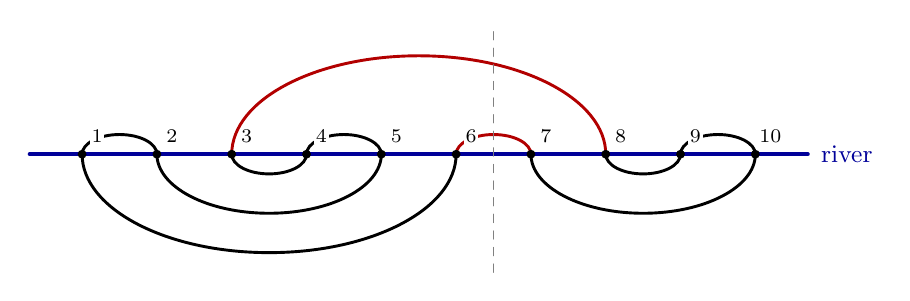
\begin{tikzpicture}[x=0.95cm,y=0.5cm,line cap=round]
  \draw[blue!60!black,line width=1.5pt] (0.3,0)--(10.7,0);
  \node[blue!60!black,anchor=west] at (10.75,0) {\small river};
  \begin{scope}[line width=1.05pt]
    \draw (1,0) arc[start angle=180,end angle=0,radius=0.5];
    \draw[red!70!black] (3,0) arc[start angle=180,end angle=0,radius=2.5];
    \draw (4,0) arc[start angle=180,end angle=0,radius=0.5];
    \draw[red!70!black] (6,0) arc[start angle=180,end angle=0,radius=0.5];
    \draw (9,0) arc[start angle=180,end angle=0,radius=0.5];
    \draw (1,0) arc[start angle=180,end angle=360,radius=2.5];
    \draw (2,0) arc[start angle=180,end angle=360,radius=1.5];
    \draw (3,0) arc[start angle=180,end angle=360,radius=0.5];
    \draw (7,0) arc[start angle=180,end angle=360,radius=1.5];
    \draw (8,0) arc[start angle=180,end angle=360,radius=0.5];
  \end{scope}
  \draw[gray,dashed] (6.5,-3)--(6.5,3.2);
  \foreach \k in {1,...,10} {\fill (\k,0) circle[radius=1.6pt]; \node[fill=white,inner sep=0.6pt,font=\scriptsize] at (\k+0.2,0.45) {\k};}
\end{tikzpicture}
\caption{A meander of order $5$ with a cut at $m=3$ (dashed line, gap $6$). No lower arch passes
over the gap; above it there is the short arch $6$--$7$ and one other arch, $3$--$8$ (both red).
Replacing these two arches by $3$--$6$ and $7$--$8$ splits the road into the running example of
Figure~\ref{fig:running} on crossings $1$--$6$ and a meander of order $2$ on crossings $7$--$10$.}
\label{fig:cut}
\end{figure}

\subsection{Prime meanders}

A meander is \emph{prime} if it has no cut. By Theorem~\ref{thm:cuts} and induction on the smallest
cut, every meander is a product $Q_1\cdot Q_2\cdots Q_k$ of primes in exactly one way, and the
product is associative. With $P_n$ the number of prime meanders of order $n$,
$\mathcal M(z)=\sum_{n\ge1}M_nz^n$ and $\mathcal P(z)=\sum_{n\ge1}P_nz^n$, this says
\[ 1+\mathcal M(z)\;=\;\frac1{1-\mathcal P(z)} . \]
The first values are $P_n=1,1,5,27,175,1255,9699,79253,676429,\ldots$, and $P_{32}/M_{32}=0.794$.
Write $U=\sum_n u_n=\mathcal M(1/\mu)$, which is finite by Theorem~\ref{thm:sumu} below. Then
$\mathcal P(1/\mu)=U/(1+U)\le1/5$. In the language of renewal theory, $(u_n)$ is a \emph{transient}
renewal sequence: a meander is a sequence of prime blocks, and the weights $P_n\mu^{-n}$ of the
possible blocks add up to less than one. That a positive fraction of meanders is prime is not
proved.

\subsection{The sum of \texorpdfstring{$u_n$}{u\_n}}

Let $X_N$ be the number of meanders of order $N$ with one marked exterior upper arch (one not
enclosed by another upper arch), so that $M_N\le X_N\le NM_N$. By reflection in the river, $X_N$ also counts meanders with a marked exterior
lower arch.

\begin{theorem}\label{thm:sumu}
$\sum_{n\ge1}u_n\le1/4$.
\end{theorem}

\begin{proof}
Two facts are needed. First, the gaps other than the two ends over which no lower arch passes are
exactly the gaps between consecutive exterior lower arches, so a meander with $\eta$ exterior lower arches has $\eta-1$ of them.
Second, the meanders of order $N$ in which no lower arch and exactly two upper arches pass over gap
$2m$ number exactly $X_mX_{N-m}$. Indeed, if the two upper arches are $\{p,r\}$ and $\{p',r'\}$ with
$p<p'\le2m<r'<r$, replacing them by $\{p,p'\}$ and $\{r',r\}$ gives a meander on each side, each with a
marked exterior arch, and this is reversible; the case $p'=2m$, $r'=2m+1$ is a cut.

Counting only the gaps over which no lower arch and exactly two upper arches pass, we get
\[ X_N-M_N\;=\;\sum_\Gamma(\eta(\Gamma)-1)\;\ge\;\sum_{m=1}^{N-1}X_mX_{N-m}, \]
where the sum is over meanders $\Gamma$ of order $N$ and $\eta(\Gamma)$ is the number of exterior lower
arches.
With $\mathcal X(z)=\sum_nX_nz^n$ this says that $\mathcal X-\mathcal X^2-\mathcal M$ has
nonnegative coefficients. For $0\le z<1/\mu$ all three series converge, and
$\mathcal M(z)\le\mathcal X(z)-\mathcal X(z)^2\le1/4$. Letting $z$ increase to $1/\mu$ gives
$\sum_nM_n\mu^{-n}\le1/4$ by monotone convergence.
\end{proof}

In particular $u_n\to0$, and for every $\xi\in(0,1]$ at most $N^\xi/4$ of the $n\le N$ have
$u_n>n^{-\xi}$. From the exact counts and $\mu\le12.2970$, $U\ge\sum_{n\le32}M_n\,12.297^{-n}>0.1032$, so
\[ 0.1032\;\le\;U\;\le\;0.25 . \]
A numerical estimate, which assumes the power law~\eqref{eq:law} for the tail, is $U\approx0.1037$.

\subsection{The number of cuts}

By~\eqref{eq:cutprob} the expected number of cuts of a random meander of order $N$ is
\[ \mathbb E_N[\#\text{cuts}]\;=\;\sum_{m=1}^{N-1}\frac{M_mM_{N-m}}{M_N}. \]
Every cut is a gap over which no lower arch passes, so the number of cuts is at most $\eta-1$, where $\eta$ is the number of exterior lower arches. The mean
number of exterior upper arches, which equals the mean number of exterior lower arches, is
$X_N/M_N$, and a short surgery at the marked exterior arch shows $2X_N\le M_{N+1}$~\cite{Repo}. Hence
\begin{equation}\label{eq:cutmean}
\mathbb E_N[\#\text{cuts}]\;\le\;\frac{M_{N+1}}{2M_N}-1\;\le\;\frac{R_\star}2-1 ,
\end{equation}
which is bounded by Theorem~\ref{thm:ratio}. The exact values are $0.338$, $0.270$ and $0.245$ at
$N=10$, $20$ and $32$, decreasing (Table~\ref{tab:cuts}).

\subsection{Cuts away from the ends}

\begin{proposition}\label{prop:cutbound}
There is a constant $C_{\mathrm c}$ such that for all $N\ge2$ and $1\le k\le N-1$, with
$s=\min(k,N-k)$,
\[ \Pr_N(\text{cut at }k)\;\le\;C_{\mathrm c}\,s^{-1/4}\sqrt{\log(s+1)} . \]
\end{proposition}

\begin{proof}[Key idea]
Write $\psi(k)=M_kM_{N-k}/M_N$, the probability of a cut at $k$; it is symmetric, so let $k\le N/2$.
Moving the cut by $t$ positions changes $\log\psi$ by a difference of two sums of $t$ terms
$\log(M_{i+1}/(\mu M_i))$, since the factors $\mu$ cancel. By Theorem~\ref{thm:rate} each term is at
most $\delta(i)=2C_{\mathrm r}\,i^{-1/4}\sqrt{\log(i+1)}$ in absolute value, with all indices at least
$k/2$. So for $t_0=\lfloor1/\delta(\lceil k/2\rceil)\rfloor$, about $k^{1/4}$, there are $t_0+1$
positions where the probability of a cut is at least $e^{-2}\psi(k)$. Their sum is at most
$\mathbb E_N[\#\text{cuts}]$, which is bounded by~\eqref{eq:cutmean}, so
$\psi(k)=O(\delta(\lceil k/2\rceil))$. Bounded $k$ are handled by enlarging the constant.
\end{proof}

Intuitively, the probability of a cut is nearly constant over stretches of about $s^{1/4}$
positions, and the total over all positions is bounded. So no neck far from both ends carries a positive fraction of meanders. Under the power law the true order is
$(N/(k(N-k)))^{\alpha}$, much smaller. The bound is not summable over positions, and a better ratio
rate would not make it summable, so it does not settle whether the cuts in the middle carry vanishing
total probability (Section~\ref{sec:subexp}).

\subsection{Near-cuts}\label{sec:nearcuts}

A cut is a very special neck. A meander of order $2m$ can also be nearly split at the middle in looser
ways. These looser events are the ones that remain visible when a large random meander is rescaled
to a continuum picture, as in Paper~D~\cite{PaperD}. Two results compare them with exact cuts.

\emph{Zero defect.} Say that a meander of order $2m$ is \emph{split at the middle} if its first $2m$
crossings form one stretch of consecutive crossings along the road. On a closed road, a set of
crossings is one stretch exactly when two road arches leave it, so this is the event that exactly two
arches pass over gap $2m$. Both arches are upper or both are lower, by parity, and the count in the
proof of Theorem~\ref{thm:sumu} gives $X_m^2$ for each case.

\begin{proposition}[zero defect]\label{prop:zerodefect}
$\Pr_{2m}(\text{split at the middle})=2X_m^2/M_{2m}$ exactly. Consequently, since
$M_m^2/M_{2m}=e^{-D(m)}$,
\[ 2e^{-D(m)}\;\le\;\Pr_{2m}(\text{split at the middle})\;\le\;\tfrac12R_\star^2\,e^{-D(m)} . \]
\end{proposition}

The inequalities follow from $M_m\le X_m\le M_{m+1}/2\le R_\star M_m/2$. So a split at the middle is a cut
at the middle up to a bounded factor: given a split, the probability of an exact cut is at least
$2/R_\star^2$.

\emph{Bounded defect.} More generally, say the first $2m$ crossings have \emph{defect at most $K$} if
they differ in at most $K$ crossings from some stretch of $2m$ consecutive crossings along the road.
Such a meander has a \emph{near-cut} at the middle.
Each changed crossing adds at most two road arches leaving the set, so at most $2+2K$ arches pass over
gap $2m$. The next result bounds such meanders by exact products.

\begin{proposition}[linear-record completion]\label{prop:linrec}
For all $m,n\ge1$ and even $w\ge2$, the number of meanders of order $m+n$ in which at most $w$ arches
pass over gap $2m$ is at most $(64R_\star^3)^w M_mM_n$.
\end{proposition}

\begin{proof}[Key idea]
Suppose exactly $w$ arches pass over the gap, $w_\uparrow$ upper and $w_\downarrow$ lower; smaller numbers are handled
in the same way. Cut at the gap. The left half has $2m$ crossings and $w$ loose ends. Append
$w$ new crossings on the right and join the loose ends to them in nested order; this closes the half
into a system of at most $w$ closed roads, each of which meets the new crossings. Then merge the roads
from left to right along the new crossings: at each of the $w-1$ steps, either the next new crossing
is already on the current road, or one of three local moves joins the two roads, adding at most two
crossings. The record of the whole merge is a word of length $w-1$ in four letters, one letter per
step. Because the steps follow a fixed left-to-right schedule, the word determines where each move
happened, so the half is recovered from the completed meander and the word. This gives at most $4^{w-1}R_\star^{3w/2}M_m$ left halves with given $w_\uparrow$ and $w_\downarrow$, the factor
$R_\star^{3w/2}$ paying for the at most $3w/2$ extra orders. The same holds on the right, and the two
halves are glued across the gap in only one way.
\end{proof}

\begin{corollary}\label{cor:defect}
For every $K\ge0$,
\[ e^{-D(m)}\;\le\;\Pr_{2m}(\text{defect at most }K)\;\le\;(64R_\star^3)^{2K+2}\,e^{-D(m)} . \]
\end{corollary}

So near-cuts with defect $K$ are at most a factor $e^{O(K+1)}$ more likely than exact cuts. For a
slowly growing defect, $K=o(\log m)$, the two probabilities agree up to a factor $m^{o(1)}$, so they
decay with the same power of $m$ if either decays like a power.

%%%%%%%%%%%%%%%%%%%%%%%%%%%%%%%%%%%%%%%%%%%%%%%%%%%%%%%%%%%%%%%%%%%%%%%%
\section{Meanders with bounded labels}\label{sec:band}
%%%%%%%%%%%%%%%%%%%%%%%%%%%%%%%%%%%%%%%%%%%%%%%%%%%%%%%%%%%%%%%%%%%%%%%%

For all meanders the exponent is out of reach. For one natural subfamily both the growth rate and the
exponent can be found exactly, and the answer shows a mechanism that is believed to produce a power
law in general: a walk confined to a wedge.

\subsection{Labels}

In this section $m$ is the order of a meander. Give each crossing $i<2m$ an integer label $\varphi_i$
so that along every arch above the river the label drops by one from left to right, and along every
arch below the river it rises by one. Precisely: $\varphi_1=0$, and $\varphi_y=\varphi_x-1$ for every
upper arch $\{x,y\}$ with $x<y<2m$, and $\varphi_y=\varphi_x+1$ for every lower arch $\{x,y\}$ with
$x<y<2m$; the two arches at the last crossing $2m$ are left out. Removing them leaves the road as a
single path through crossings $1,\ldots,2m-1$, so these rules determine the labels uniquely.
Intuitively, $\varphi_i$ counts the half turns of the road on its way from crossing $1$ to crossing
$i$, with opposite signs above and below the river. For a meander, labels of neighboring crossings
along the river differ by one. Conversely, a pair of arch systems is a meander if and only if it has a
labeling that obeys these rules and in which neighboring labels differ by one. Paper~B explains these
labels~\cite{PaperB}. In the running example of Figure~\ref{fig:running} the labels of crossings $1$
to $5$ are $0,-1,0,1,0$.

Let $M^{[-1,2]}_m$ be the number of meanders of order $m$ whose labels all lie in $\{-1,0,1,2\}$. It
starts $1,2,7,31,161,932,5841,38891$. The labels depend on which crossing is first and which is last,
so this is a family of meanders with distinguished ends, not closed under all symmetries of the
picture.

\subsection{The growth rate}

Let $x_0=0.9175433408\ldots$ be the positive root of $4x^4=2x+1$ and
\[ \Lambda\;=\;(1+2x_0)(1+x_0)^2\;=\;10.4245356612\ldots, \]
the larger real root of the irreducible polynomial $16x^4-112x^3-520x^2-536x+25$.

\begin{theorem}[growth rate]\label{thm:bandgrowth}
There is a constant $C_\Lambda$ such that for every $m\ge1$
\[ \Lambda^{m-1}e^{-C_\Lambda\sqrt m}\;\le\;M^{[-1,2]}_m\;\le\;\Lambda^{m-1}. \]
\end{theorem}

\begin{proof}[Key idea]
Read the crossings from left to right. After crossing $j$ the state is the current label together with
the labels of the upper arches and of the lower arches that are still open, that is, started but not
yet closed. The open arches on each side are closed in last-in-first-out order, so they form a stack.
Since the labels take only four values, each stack is a word in a finite alphabet, and the reading
process is a machine with two stacks and finitely many control states. This machine has an explicit
eigenfunction of product form, with one weight for each stack entry below the top, and
normalizing by it turns the count into a probability: $M^{[-1,2]}_m=\Lambda^{m-1}$ times the
probability that an explicit Markov chain, reading one crossing at a time, is back in its starting
state after $2m-2$ crossings without having been killed (stopped) on the way. The upper bound follows
at once. For the lower bound, consider the chain without the constraint that a stack cannot go below
empty. It has an invariant law of product form, and under it two explicit martingales show that with
probability at least $1/2$ the chain stays for $t$ steps within windows of length about $\sqrt t$ at
the tops of the two stacks. Building such windows from the start and removing them at the end costs a
factor $e^{-O(\sqrt t)}$.
\end{proof}

\subsection{The exponent}

Let $\theta=\arccos\big((1+2x_0)/(3+4x_0)\big)=1.13179\ldots$, which is $64.8468\ldots$ degrees, and
\[ \alpha_{\mathrm b}\;=\;1+\frac{\pi}{\theta}\;=\;3.7757713065\ldots . \]

\begin{theorem}[exponent]\label{thm:bandexp}
For every $\epsilon>0$ there are $c_\epsilon,C_\epsilon>0$ such that for every $m\ge2$
\[ c_\epsilon\,\Lambda^m m^{-\alpha_{\mathrm b}-\epsilon}\;\le\;M^{[-1,2]}_m\;\le\;C_\epsilon\,\Lambda^m m^{-\alpha_{\mathrm b}+\epsilon}. \]
That is, $M^{[-1,2]}_m=\Lambda^m m^{-\alpha_{\mathrm b}+o(1)}$.
\end{theorem}

Both numbers are explicit, and neither is rational: $\Lambda$ is algebraic of degree four, and
$\alpha_{\mathrm b}$ is irrational, indeed transcendental. For the irrationality, $u=2\cos\theta$ is a
root of the polynomial
\[ 113u^4-312u^3+312u^2-128u+16 , \]
obtained by substituting $x_0=(2-3u)/(4u-4)$ into $4x_0^4-2x_0-1=0$. It is irreducible: its reduction
modulo $3$, made monic, is $X^4-X-1$, which has no factor of degree one or two over the field with
three elements. So the monic minimal polynomial of $u$ has the constant term $16/113$, and $u$ is not an
\emph{algebraic integer}, a root of a monic polynomial with integer coefficients. If $\theta/\pi$ were
rational, $e^{i\theta}$ would be a root of unity and $u=e^{i\theta}+e^{-i\theta}$ would be an
algebraic integer. Hence $\theta/\pi$ is irrational, and so is $\alpha_{\mathrm b}=1+\pi/\theta$. Since
$e^{i\theta}$ is algebraic, the Gelfond--Schneider theorem then makes $\theta/\pi$, and with it
$\alpha_{\mathrm b}$, transcendental. The sharp form $M^{[-1,2]}_m\asymp\Lambda^mm^{-\alpha_{\mathrm b}}$, with
bounded ratio, is not proved, and no closed formula for the counts is known.

\subsection{The generating function}

A power series is \emph{D-finite} if it satisfies a nonzero linear differential equation whose
coefficients are polynomials. Algebraic power series are D-finite, but many D-finite series are not
algebraic. The generating function of the bounded-label family is in neither class.

\begin{corollary}\label{cor:bandnondfinite}
The generating function
\[ F_{\mathrm b}(z)\;=\;\sum_{m\ge1}M^{[-1,2]}_m z^m \]
is not D-finite, even with complex polynomial coefficients. In particular, it is not algebraic.
\end{corollary}

\begin{proof}
By the previous subsection, $\alpha_{\mathrm b}$ is irrational. Choose an integer $k$ with
$k+1>\alpha_{\mathrm b}$. The coefficient bounds of Theorem~\ref{thm:bandexp} give
\begin{equation}\label{eq:bandradial}
\lim_{r\downarrow0}\frac{\log F_{\mathrm b}^{(k)}\big((1-r)/\Lambda\big)}{\log(1/r)}\;=\;k+1-\alpha_{\mathrm b} .
\end{equation}
To see this, note that the $k$th derivative of $z^m$ is ${m(m-1)\cdots(m-k+1)}\,z^{m-k}$, and this
factor is of order $m^k$ for large $m$. So for each small $\epsilon>0$ the
positive series $F_{\mathrm b}^{(k)}((1-r)/\Lambda)$ lies, up to bounded factors and finitely many bounded
terms, between $\sum_m m^{k-\alpha_{\mathrm b}-\epsilon}(1-r)^m$ and $\sum_m m^{k-\alpha_{\mathrm b}+\epsilon}(1-r)^m$.
These sums are of order $r^{-(k+1-\alpha_{\mathrm b}\mp\epsilon)}$, which tends to infinity. Taking
logarithms and letting $\epsilon$ decrease to zero proves~\eqref{eq:bandradial}.

Suppose now that $F_{\mathrm b}$ were D-finite. Its coefficients are rational, so an equation with
complex coefficients can be replaced by one with rational coefficients: for a fixed order and degree,
the coefficients of the equation solve a system of homogeneous linear equations with rational
coefficients, and such a system with a nonzero complex solution has a nonzero rational one. Since the
coefficients of $F_{\mathrm b}$ are integers bounded by $16^m$, it is then a \emph{G-function}, a D-finite
series whose coefficients satisfy standard arithmetic growth bounds. The Andr\'e--Chudnovsky--Katz
theorem says that the minimal equation of a G-function has only regular singularities, with rational
exponents~\cite[Theorem~6]{FischlerRivoal2014}. By~\eqref{eq:bandradial}, $1/\Lambda$ is a singular point.
So near $1/\Lambda$ the function and its derivatives are finite sums of rational powers of $1/\Lambda-z$
times powers of $\log(1/\Lambda-z)$ times analytic functions. After equal powers are combined, the
first nonzero term shows that the limit in~\eqref{eq:bandradial} is rational. This contradicts the
irrationality of $\alpha_{\mathrm b}$. Finally, every algebraic power series is D-finite.
\end{proof}

The proof uses the coefficient bounds of Theorem~\ref{thm:bandexp} with arbitrary $\epsilon$; it does not
need the sharp form $M^{[-1,2]}_m\asymp\Lambda^mm^{-\alpha_{\mathrm b}}$. It also needs nothing about other
singularities on the circle $|z|=1/\Lambda$, because all estimates are made on the positive real axis.

\subsection{The wedge}

The following heuristic explains why the exponent is $1+\pi/\theta$; the proofs make it rigorous. Let $h_\uparrow(j)$ and $h_\downarrow(j)$ be the numbers of
upper and lower arches still open after crossing $j$: the heights of the two stacks. A meander starts
and ends with both heights zero, and in between neither is negative. So the pair of heights is a walk
in the quarter plane that starts and ends at the corner.

For the chain of Theorem~\ref{thm:bandgrowth}, the two heights after $t$ steps, rescaled by $\sqrt t$,
converge to a planar Brownian motion whose two coordinates have correlation
\[ \rho\;=\;-\frac{1+2x_0}{3+4x_0}\;=\;-0.42504\ldots . \]
A linear change of coordinates turns this Brownian motion into a standard one and the quarter plane
into a wedge of angle $\theta=\arccos(-\rho)$. The correlation is negative: when one stack grows, the
other tends to shrink, so it is harder for both to stay positive, and the wedge is narrower than a
right angle.

For standard Brownian motion in a wedge of angle $\theta$, started at distance one from the corner, the
probability of staying inside for time $t$ decays like $t^{-\pi/(2\theta)}$~\cite{DW}. A meander asks for
more: an excursion from the corner back to the corner. That costs $t^{-\pi/(2\theta)}$ for the first
half, the same for the second half read backward, and $t^{-1}$ for ending in a bounded region near the
corner, as for any two-dimensional walk. Altogether $t^{-1-\pi/\theta}=t^{-\alpha_{\mathrm b}}$, and
$t=2m-2$ is proportional to the order. Figure~\ref{fig:wedge} shows the picture.

\begin{figure}[t]
\centering
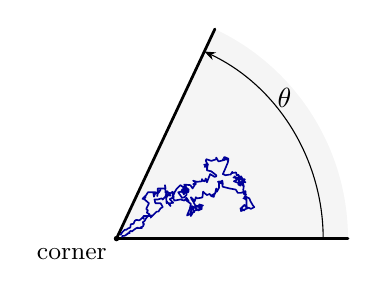
\begin{tikzpicture}[scale=0.7,line cap=round,line join=round]
  \fill[gray!8] (0,0)--(4.2,0) arc[start angle=0,end angle=64.846841,radius=4.2]--cycle;
  \draw[line width=1pt] (0,0)--(4.2,0);
  \draw[line width=1pt] (0,0)--(64.846841:4.2);
  \draw[-{Stealth[length=4pt]}] (3.75,0) arc[start angle=0,end angle=64.846841,radius=3.75];
  \node at (40:3.98) {$\theta$};
  \draw[blue!60!black,line width=0.6pt] plot coordinates {(0.10,0.03) (0.11,0.05) (0.14,0.05) (0.17,0.06) (0.18,0.08) (0.20,0.08) (0.21,0.10) (0.24,0.10) (0.23,0.12) (0.26,0.14) (0.28,0.13) (0.33,0.17) (0.36,0.19) (0.39,0.20) (0.38,0.19) (0.46,0.19) (0.43,0.20) (0.48,0.22) (0.50,0.27) (0.49,0.24) (0.49,0.24) (0.48,0.30) (0.51,0.32) (0.53,0.36) (0.60,0.44) (0.55,0.47) (0.57,0.51) (0.54,0.54) (0.59,0.64) (0.51,0.71) (0.50,0.71) (0.53,0.76) (0.47,0.72) (0.54,0.79) (0.57,0.84) (0.64,0.84) (0.71,0.84) (0.68,0.76) (0.67,0.82) (0.68,0.83) (0.73,0.82) (0.80,0.88) (0.78,0.86) (0.77,0.84) (0.75,0.82) (0.74,0.77) (0.75,0.91) (0.77,0.91) (0.89,0.91) (0.88,0.97) (0.89,0.83) (0.93,0.84) (0.90,0.86) (0.90,0.82) (0.92,0.86) (0.98,0.78) (0.93,0.79) (1.02,0.85) (1.02,0.75) (1.05,0.69) (1.11,0.70) (1.16,0.71) (1.23,0.69) (1.26,0.72) (1.27,0.74) (1.31,0.68) (1.27,0.69) (1.35,0.63) (1.33,0.54) (1.28,0.42) (1.40,0.48) (1.41,0.48) (1.37,0.59) (1.48,0.52) (1.48,0.51) (1.55,0.54) (1.52,0.54) (1.52,0.57) (1.45,0.58) (1.37,0.56) (1.34,0.45) (1.35,0.41) (1.40,0.50) (1.54,0.55) (1.50,0.62) (1.57,0.60) (1.55,0.60) (1.55,0.57) (1.49,0.59) (1.43,0.60) (1.41,0.64) (1.36,0.73) (1.37,0.70) (1.35,0.75) (1.42,0.68) (1.44,0.75) (1.46,0.73) (1.53,0.74) (1.56,0.75) (1.57,0.85) (1.58,0.85) (1.58,0.84) (1.64,0.79) (1.69,0.81) (1.72,0.77) (1.77,0.76) (1.75,0.76) (1.78,0.80) (1.72,0.78) (1.79,0.82) (1.81,0.91) (1.82,0.85) (1.86,0.92) (1.86,1.04) (1.86,1.02) (1.92,1.05) (1.93,0.99) (1.89,1.02) (1.92,1.01) (1.84,1.03) (1.93,0.99) (1.92,0.96) (1.93,0.94) (2.05,0.91) (2.16,0.89) (2.17,0.88) (2.20,0.83) (2.26,0.83) (2.34,0.86) (2.34,0.75) (2.35,0.76) (2.41,0.73) (2.43,0.68) (2.47,0.61) (2.50,0.57) (2.44,0.54) (2.40,0.56) (2.26,0.50) (2.25,0.55) (2.32,0.51) (2.26,0.55) (2.32,0.61) (2.37,0.55) (2.36,0.60) (2.36,0.71) (2.36,0.70) (2.32,0.73) (2.30,0.73) (2.30,0.73) (2.32,0.73) (2.36,0.71) (2.32,0.75) (2.35,0.80) (2.31,0.81) (2.30,0.89) (2.31,0.95) (2.30,0.99) (2.29,0.96) (2.30,1.06) (2.26,1.13) (2.22,1.03) (2.21,0.98) (2.25,0.96) (2.24,1.01) (2.32,1.08) (2.33,1.07) (2.17,1.09) (2.14,1.13) (2.21,1.07) (2.20,1.11) (2.17,1.10) (2.12,1.11) (2.18,1.11) (2.22,1.06) (2.24,1.01) (2.25,1.02) (2.31,1.03) (2.34,1.02) (2.27,1.08) (2.29,1.06) (2.29,1.00) (2.27,0.99) (2.30,0.98) (2.29,0.98) (2.13,1.04) (2.19,1.07) (2.23,1.12) (2.21,1.16) (2.18,1.15) (2.17,1.20) (2.10,1.19) (2.10,1.21) (2.07,1.16) (2.04,1.16) (1.98,1.15) (1.93,1.17) (1.97,1.26) (2.02,1.38) (2.03,1.43) (2.01,1.43) (1.95,1.47) (1.96,1.48) (2.03,1.45) (1.93,1.44) (1.97,1.43) (1.85,1.40) (1.81,1.47) (1.81,1.44) (1.72,1.41) (1.63,1.44) (1.62,1.41) (1.65,1.35) (1.60,1.30) (1.65,1.32) (1.59,1.34) (1.66,1.35) (1.65,1.32) (1.64,1.27) (1.65,1.31) (1.64,1.24) (1.72,1.22) (1.81,1.15) (1.81,1.13) (1.78,1.12) (1.70,1.17) (1.64,1.02) (1.62,1.09) (1.60,1.04) (1.57,1.05) (1.55,1.08) (1.55,1.04) (1.46,1.03) (1.39,1.05) (1.42,1.03) (1.44,0.99) (1.39,0.99) (1.43,0.99) (1.38,0.91) (1.34,0.97) (1.23,0.98) (1.25,0.85) (1.22,0.80) (1.25,0.88) (1.26,0.95) (1.24,0.95) (1.23,0.86) (1.27,0.84) (1.23,0.89) (1.20,0.90) (1.18,0.87) (1.20,0.83) (1.22,0.86) (1.29,0.84) (1.27,0.85) (1.31,0.86) (1.25,0.94) (1.26,0.94) (1.24,0.94) (1.30,0.84) (1.31,0.89) (1.27,0.92) (1.27,0.91) (1.27,0.79) (1.23,0.75) (1.19,0.74) (1.12,0.84) (1.23,0.86) (1.22,0.88) (1.24,0.91) (1.16,0.97) (1.09,0.90) (1.06,0.85) (1.03,0.78) (1.04,0.75) (0.97,0.72) (0.97,0.71) (1.03,0.65) (0.96,0.64) (0.98,0.59) (0.91,0.68) (0.91,0.64) (0.90,0.76) (0.96,0.83) (0.91,0.75) (0.89,0.79) (0.92,0.80) (0.84,0.71) (0.82,0.73) (0.75,0.71) (0.69,0.71) (0.70,0.66) (0.71,0.64) (0.80,0.64) (0.82,0.61) (0.84,0.57) (0.80,0.55) (0.76,0.49) (0.73,0.49) (0.62,0.38) (0.65,0.42) (0.60,0.41) (0.53,0.41) (0.49,0.41) (0.49,0.36) (0.49,0.40) (0.45,0.36) (0.44,0.35) (0.41,0.33) (0.36,0.34) (0.33,0.32) (0.31,0.27) (0.26,0.26) (0.25,0.20) (0.20,0.18) (0.18,0.16) (0.15,0.16) (0.12,0.13) (0.10,0.11) (0.09,0.09) (0.07,0.07)};
  \fill (0,0) circle[radius=1.4pt];
  \node[below left,font=\small] at (0,0) {corner};

\end{tikzpicture}
\caption{Schematic: after a linear change of coordinates the two stack heights move like a planar
Brownian motion in a wedge of angle $\theta$, and a meander is an excursion from the corner back to the
corner. Here $\theta\approx64.85^\circ$. The path drawn is illustrative, not a sample.}
\label{fig:wedge}
\end{figure}

Two checks make the formula plausible. Without the requirement of a single loop, the upper and lower
arch systems are independent, the heights are independent, $\rho=0$, $\theta=\pi/2$, and the exponent
is $1+2=3$; indeed the number of pairs of arch systems is $\mathrm{Cat}_n^2\approx16^n/(\pi n^3)$. For the
narrower band of labels $\{-1,0,1\}$, the counts $1,2,6,22,92,422,2074,\ldots$ are the Baxter
numbers. Chung, Graham, Hoggatt and Kleiman gave an explicit formula for them~\cite{CGHK}, from which
they grow like a constant times $8^n n^{-4}$;
there $\rho=-1/2$, $\theta=\pi/3$ and $1+\pi/\theta=4$. The identification with the Baxter numbers is
from the literature and was checked here only on small orders, not proved.

The main difficulty in the proofs is that the heights are not a random walk with independent steps:
the chain is Markov only on its full state, two words of unbounded length. The proofs replace
independence by stationarity under the invariant law, and the lower bound also uses that the chain
reversed in time is again an explicit two-stack machine.

For all meanders the stacks are unbounded in both directions and no finite description of this kind
is known. Whether the exponent of all meanders arises from a wedge in a similar way is the question
behind Papers~A and~D~\cite{PaperA,PaperD}.

%%%%%%%%%%%%%%%%%%%%%%%%%%%%%%%%%%%%%%%%%%%%%%%%%%%%%%%%%%%%%%%%%%%%%%%%
\section{What would improve the bounds}\label{sec:improve}
%%%%%%%%%%%%%%%%%%%%%%%%%%%%%%%%%%%%%%%%%%%%%%%%%%%%%%%%%%%%%%%%%%%%%%%%

Theorem~\ref{thm:main} leaves the loss $L(n)$ between about $\log n$ and $C\sqrt n$. This section
states what would lower the upper estimate $C\sqrt n$, why some natural routes cannot, and what
weaker targets remain. The propositions and the argument that gluing cannot help have complete
written proofs, which have not been checked independently; the expected value of $\beta$ is a
heuristic.

\subsection{Short separators for a fraction of meanders}

The proof of the lower bound applies one separator with about $\sqrt N$ ports to every meander. A
separator with fewer ports may exist only for some meanders; then the argument must also pay for how
rare these meanders are.

\begin{proposition}[fraction criterion]\label{prop:fraction}
Let $0<\tau<1$ and $c_{\mathrm f}>0$. Suppose that for all large $N$ a fraction at least
$e^{-c_{\mathrm f}N^\tau}$ of the meanders of order $N$ have a separator with at most
$c_{\mathrm f}N^\tau$ ports whose two disks each contain between $N/2$ and $3N/2$ of the $2N$
crossings. Then $L(n)\le K_{\mathrm f}\,n^\tau$ for all $n$, for some constant $K_{\mathrm f}$.
\end{proposition}

\begin{proof}[Key idea]
Run the proof of Proposition~\ref{prop:reverse} on these meanders only. Their number is at least
$e^{-c_{\mathrm f}N^\tau}M_N$ and at most a polynomial times $e^{2c_\Omega c_{\mathrm f}N^\tau}\max M_aM_b$,
so $L(a)+L(b)\le L(N)+B'N^\tau$. The descent of Section~\ref{sec:descent} goes through with
$N^{\tau-1}$ in place of $N^{-1/2}$, because the geometric sums still converge.
\end{proof}

With $\tau=1/2$ and fraction one this is the lower bound of Theorem~\ref{thm:main}. The criterion
allows separators of any shape. For example, if every face of the map can be reached from one fixed
face by crossing at most $\omega$ edges, the map has a balanced separator with at most $2\omega+1$ ports.

\subsection{Shallow meanders}

The simplest balanced cut is a vertical line through the middle gap of the river. It always exists,
it splits the crossings evenly, and its ports are the arches that pass over the gap, so its cost
depends on how many arches do. Say that an arch system has \emph{depth} at most $d$ if no point lies
under more than $d$ of its arches, and let $M^{(d)}_n$ count meanders of order $n$ whose upper and
lower arch systems both have depth at most $d$. We call these \emph{shallow} meanders.

\begin{proposition}[depth criterion]\label{prop:depth}
Suppose that for some $K_{\mathrm d}$ and $\beta>0$
\[ M^{(d)}_n\;\ge\;\mu^n\exp\!\big(-K_{\mathrm d}\,n\,d^{-\beta}-K_{\mathrm d}\,d\big)\qquad\text{for all }n,d\ge1 .\]
Then $L(m)\le K_{\mathrm d}'\,m^{1/(1+\beta)}$ for all $m$, for some constant $K_{\mathrm d}'$.
\end{proposition}

\begin{proof}
In a meander of depth at most $d$, at most $2d$ arches pass over the middle gap. By
Proposition~\ref{prop:linrec}, $M^{(d)}_{2m}\le e^{2B_{\mathrm{lin}}d}M_m^2$ with $B_{\mathrm{lin}}=\log(64R_\star^3)$.
With the hypothesis at $n=2m$,
\[ 2m\log\mu-2K_{\mathrm d}md^{-\beta}-K_{\mathrm d}d\;\le\;2B_{\mathrm{lin}}d+2\log M_m , \]
so $L(m)\le K_{\mathrm d}\,m\,d^{-\beta}+(B_{\mathrm{lin}}+K_{\mathrm d}/2)\,d$.
Take $d=\lceil m^{1/(1+\beta)}\rceil$.
\end{proof}

The exponent $1/(1+\beta)$ is below $1/2$ exactly when $\beta>1$. So shallow meanders improve on the
square root if and only if confining a meander to depth $d$ costs less than $d^{-1}$ per crossing in
the exponent.

\emph{Gluing short meanders never helps.} Let $\mu_d=\lim_n(M^{(d)}_n)^{1/n}$ be the growth rate of
shallow meanders. The only unconditional lower bounds for $M^{(d)}_n$ come from building shallow
meanders out of short ones, by products. A meander of order $n_1\le d$ has depth at most $n_1$, and a
product of many of them, combined in a balanced way, adds only a few levels of nesting. This gives
$\log(\mu/\mu_d)\lesssim L(n_1)/n_1$ with $n_1\approx d$. If $L(n_1)=O(n_1^{\tau})$, that is $\beta=1-\tau$, and Proposition~\ref{prop:depth} returns the exponent
$1/(2-\tau)$. Since
\[ \frac1{2-\tau}-\tau\;=\;\frac{(1-\tau)^2}{2-\tau}\;\ge\;0, \]
the exponent never improves; from $\tau=1/2$ it gives $2/3$, worse than the square root. A proof along
these lines must produce long, thin meanders that are not concatenations of short ones.

\emph{What is expected.} Heuristically, $\beta\approx1.92$. Typical arch heights in large meanders, the
numbers of arches nested above a point, are predicted by a KPZ-type argument to grow like $n^\nu$ with $\nu\approx0.52$, and Monte Carlo measurements on the
closely related semi-meanders, where the river is a half-line, give $0.518$~\cite{Golinelli}. For a process whose height after $n$ steps is about
$n^\nu$, staying below height $d$ for a long time costs a factor of about
$\exp(-\mathrm{const}\cdot d^{-1/\nu})$ per step, which suggests
$\log(\mu/\mu_d)\approx\mathrm{const}\cdot d^{-1/\nu}$ and $\beta=1/\nu\approx1.92$. If so, and if the
hypothesis of Proposition~\ref{prop:depth} holds with this $\beta$, it gives $L(n)=O(n^{0.34})$. For comparison, pairs of arch systems without the
single-loop condition have $\beta=2$ exactly: those of depth at most $d$ grow like
$\sigma_d=(2\cos(\pi/(d+2)))^4$ per order, and $16-\sigma_d\approx32\pi^2/(d+2)^2$.

\emph{A cleaner sufficient condition.} The hypothesis of Proposition~\ref{prop:depth} would follow, with
$\beta$ up to $2$, from a correlation statement: that
$\mu_d/\sigma_d\ge(\mu/16)\exp(-O(d^{-\beta'}))$ for some $\beta'>1$, with uniform prefactors. In words, among pairs of arch systems of depth at most
$d$, the probability of forming a single loop decays at nearly the same exponential rate as for all
pairs. The growth rates $\mu_d$ can be computed exactly for small $d$ by transfer matrices, finite
matrices that build a shallow meander one crossing at a time, so this can be tested before a proof is attempted.

\subsection{Existence of an exponent is not easier}

One might hope to prove that some exponent exists, $u_n=n^{-\alpha+o(1)}$ for some finite $\alpha$,
without finding it. This is at least as hard as a lower bound on $M_n$ of the form $\mu^n$ times a
power of $n$: if such an $\alpha$ exists,
then $L(n)\le(\alpha+1)\log n$ for large $n$, that is $M_n\ge\mu^nn^{-\alpha-1}$. By
Corollary~\ref{cor:halving}, such a polynomial lower bound is the same as $D(m)\le\chi\log m+O(1)$ for
some $\chi$, that is, $M_{2m}=O(m^{\chi}M_m^2)$. No method in this paper gives that.

\subsection{A weaker target: subexponentiality}\label{sec:subexp}

A summable positive sequence $(a_n)$ is called \emph{subexponential} if
\[ \frac1{a_N}\sum_{m=1}^{N-1}a_ma_{N-m}\;\longrightarrow\;2\sum_na_n \qquad(N\to\infty). \]
In words, a large total is almost always made of one large part and one small part. Take $a_n=u_n$. By
\eqref{eq:cutprob} the left side is exactly $\mathbb E_N[\#\text{cuts}]$. So
\[ (u_n)\text{ is subexponential}\quad\Longleftrightarrow\quad\mathbb E_N[\#\text{cuts}]\to2U . \]
Since $\Pr_N(\text{cut at }m)\to u_m$ for each fixed $m$, by Theorem~\ref{thm:ratio}, the cuts near
the two ends already contribute $2U$ in the limit. So subexponentiality says that cuts with both sides
large carry vanishing total probability: for every $\epsilon>0$ there is $k_0$ with
$\sum_{k_0\le k\le N-k_0}\Pr_N(\text{cut at }k)\le\epsilon$ for all large $N$. Intuitively, when a large
meander has a cut, one side is almost always small.

This is a different target from a polynomial lower bound, and neither is known to imply the other. It
allows fast decay: sequences like $e^{-\sqrt n}$ are subexponential. It would have a concrete consequence. Since every meander is a sequence of primes and
$\sum u_n$ is finite, the standard theory of subexponential sequences~\cite{CNW} would give a positive limiting
fraction of prime meanders, $P_n/M_n\to(1-\mathcal P(1/\mu))^2$; the exact hypotheses of that theory
remain to be checked here. The exact data are consistent with it: $\mathbb E_N[\#\text{cuts}]$
decreases, to $0.245$ at $N=32$, while $2U\ge0.2064$ and the estimate of $U$ gives $2U\approx0.207$;
the middle part with $k_0=5$ is $0.0127$ at $N=32$ (Table~\ref{tab:cuts}). Proposition~\ref{prop:cutbound}
bounds each middle term, but its bound is not summable. What is missing is an argument that sees many
cut positions at once; local smoothness of $u_n$ alone cannot give it.

%%%%%%%%%%%%%%%%%%%%%%%%%%%%%%%%%%%%%%%%%%%%%%%%%%%%%%%%%%%%%%%%%%%%%%%%
\section{Open problems}\label{sec:open}
%%%%%%%%%%%%%%%%%%%%%%%%%%%%%%%%%%%%%%%%%%%%%%%%%%%%%%%%%%%%%%%%%%%%%%%%

\begin{enumerate}
\item \emph{A polynomial lower bound.} Prove $M_n\ge\mu^nn^{-\chi}$ for some $\chi$, equivalently
$M_{2m}=O(m^{\chi'}M_m^2)$ for some $\chi'$. This is the main gap. By Proposition~\ref{prop:linrec}, it would follow from a
lower bound, polynomial in $m$, for the probability that at most a fixed number of arches pass over
the middle gap of a meander of order $2m$. It is implied by the existence of an exponent.
\item \emph{Improving the square root.} Prove $L(n)=o(\sqrt n)$. Two routes are stated precisely: short
balanced separators for a not too small fraction of meanders (Proposition~\ref{prop:fraction}), or
the depth hypothesis of Proposition~\ref{prop:depth} with some $\beta>1$. For the second, the
correlation statement for shallow arch systems in Section~\ref{sec:improve} is a cleaner sufficient
condition that can first be tested exactly.
\item \emph{An upper bound beyond $1/n$.} Prove $u_n=O(n^{-\kappa})$ for some $\kappa>1$. Theorem~\ref{thm:threehalves} gives $3/2$ only along a subsequence. A related open
statement is $M_{n+1}\le\mu M_n$ for every $n$, which holds for $n\le31$.
\item \emph{Middle cuts.} Show that cuts with both sides large carry vanishing total probability,
that is, that $(u_n)$ is subexponential, and deduce that a positive fraction of meanders is prime.
\item \emph{Bounded labels, sharp form.} Prove
$M^{[-1,2]}_m\asymp\Lambda^mm^{-\alpha_{\mathrm b}}$, and find the exponents of wider bands of
labels. For every band of labels that contains $0$ and $1$, the corresponding family is closed under
products, so it has a growth rate, but the exponents of the wider bands are not known, nor whether they approach $\alpha_*$ as the
band widens.
\item \emph{The exponent.} Prove that $u_n=n^{-\alpha+o(1)}$ for some $\alpha$, and that
$\alpha=\alpha_*$. Paper~A explains the conjectured value~\cite{PaperA}, and Paper~D studies a
continuum counterpart~\cite{PaperD}.
\end{enumerate}

%%%%%%%%%%%%%%%%%%%%%%%%%%%%%%%%%%%%%%%%%%%%%%%%%%%%%%%%%%%%%%%%%%%%%%%%
\clearpage
\appendix
\section{Exact data}\label{app:data}
%%%%%%%%%%%%%%%%%%%%%%%%%%%%%%%%%%%%%%%%%%%%%%%%%%%%%%%%%%%%%%%%%%%%%%%%

All values below are computed from the published exact counts $M_n$ for $n\le32$: OEIS A005315~\cite{OEIS} for
$n\le28$ and~\cite{JensenGit} for $29\le n\le32$. They need no value of $\mu$. Nothing is fitted.

\begin{table}[H]
\centering
\small
\begin{tabular}{rrrr@{\hspace{1.2em}}rrr}
\toprule
$m$ & $D(m)$ & $m\,(D(m+1)-D(m))$ & $D(2m)-D(m)$ & $m$ & $D(m)$ & $m\,(D(m+1)-D(m))$\\
\midrule
$1$ & $0.6931$ & $1.6582$ & $1.6582$ & $9$ & $6.5482$ & $2.9622$\\
$2$ & $2.3514$ & $2.0014$ & $1.7902$ & $10$ & $6.8773$ & $3.0023$\\
$3$ & $3.3521$ & $2.3683$ & $1.9612$ & $11$ & $7.1776$ & $3.0361$\\
$4$ & $4.1415$ & $2.5426$ & $2.0425$ & $12$ & $7.4536$ & $3.0648$\\
$5$ & $4.7772$ & $2.6804$ & $2.1001$ & $13$ & $7.7090$ & $3.0896$\\
$6$ & $5.3133$ & $2.7781$ & $2.1403$ & $14$ & $7.9466$ & $3.1112$\\
$7$ & $5.7763$ & $2.8539$ & $2.1703$ & $15$ & $8.1689$ & $3.1302$\\
$8$ & $6.1840$ & $2.9137$ & $2.1935$ &  &  & \\
\bottomrule
\end{tabular}
\caption{The doubling defect $D(m)=\log(M_{2m}/M_m^2)=-\log\Pr_{2m}(\text{cut at }m)$. If
$u_n\sim An^{-\alpha}$, the column $D(2m)-D(m)$ tends to $\alpha\log2$, and, if the correction is also smooth,
the column $m\,(D(m+1)-D(m))$ tends to $\alpha$; for $\alpha_*$ these limits are $3.4201$ and $2.3707$. The first needs $D(m+1)$, hence
$M_{2m+2}$, and the second needs $M_{4m}$, so it stops at $m=8$.}
\label{tab:D}
\end{table}

\begin{table}[H]
\centering
\begin{tabular}{rrrrrr}
\toprule
$N$ & $\mathbb E_N[\#\text{cuts}]$ & $k_0=2$ & $k_0=3$ & $k_0=5$ & $10^4\,M_{N/2}^2/M_N$\\
\midrule
$10$ & $0.3378$ & $0.1088$ & $0.0544$ & $0.0084$ & $84.20$\\
$12$ & $0.3159$ & $0.0994$ & $0.0514$ & $0.0156$ & $49.26$\\
$16$ & $0.2876$ & $0.0858$ & $0.0445$ & $0.0178$ & $20.62$\\
$20$ & $0.2704$ & $0.0770$ & $0.0393$ & $0.0166$ & $10.31$\\
$24$ & $0.2590$ & $0.0710$ & $0.0355$ & $0.0151$ & $5.79$\\
$28$ & $0.2510$ & $0.0668$ & $0.0327$ & $0.0138$ & $3.54$\\
$32$ & $0.2451$ & $0.0636$ & $0.0306$ & $0.0127$ & $2.30$\\
\bottomrule
\end{tabular}
\caption{The expected number of cuts $\mathbb E_N[\#\text{cuts}]=\sum_{k=1}^{N-1}M_kM_{N-k}/M_N$, the
part of this sum with $k_0\le k\le N-k_0$, and the probability of a cut exactly at the middle (times
$10^4$). The total does not increase for any $N\le32$; the middle parts with $k_0=2$, $3$ and $5$
decrease for $N\ge6$, $9$ and $15$ respectively. If $(u_n)$ is subexponential (Section~\ref{sec:subexp}), the total tends to $2U\ge0.2064$.}
\label{tab:cuts}
\end{table}

The prime counts $P_n$ follow from $1+\mathcal M=1/(1-\mathcal P)$, that is
$M_n=\sum_{k=1}^{n}P_kM_{n-k}$ with $M_0=1$; $P_{32}/M_{32}=0.7938$. The ratios $M_{n+1}/M_n$ increase for
$n\le31$, from $2$ to $11.0227$.

%%%%%%%%%%%%%%%%%%%%%%%%%%%%%%%%%%%%%%%%%%%%%%%%%%%%%%%%%%%%%%%%%%%%%%%%
\section{Where the proofs are}\label{app:repo}
%%%%%%%%%%%%%%%%%%%%%%%%%%%%%%%%%%%%%%%%%%%%%%%%%%%%%%%%%%%%%%%%%%%%%%%%

All proofs, programs and data are in the project repository~\cite{Repo}, folder
\texttt{meandric/research}. ``Checked'' means that a separate, independent reading of the written
proof found no gap; the folder of that reading is given in parentheses. ``Proved'' means that a
complete proof is written but has not been checked in this way. ``Data'' means exact computation, with
no claim of proof. Nothing has been reviewed outside the project.

\begin{center}
\footnotesize
\begin{tabular}{>{\raggedright\arraybackslash}p{0.45\textwidth}>{\raggedright\arraybackslash}p{0.27\textwidth}>{\raggedright\arraybackslash}p{0.19\textwidth}}
\toprule
result & folders & status\\
\midrule
Products and cuts, primes (Theorem~\ref{thm:cuts}) & \texttt{120}; also \texttt{403} & checked (\texttt{120}, \texttt{404})\\
Ratio limit (Theorem~\ref{thm:ratio}) & \texttt{113} & checked (\texttt{113})\\
Rate in the ratio limit (Theorem~\ref{thm:rate}) & \texttt{628}, \texttt{621} & checked (\texttt{631})\\
Rate $n^{-1/4}$ (remark after Theorem~\ref{thm:rate}) & \texttt{1342}, \texttt{621} & checked (\texttt{1340})\\
Halving identity (Proposition~\ref{prop:halving}, Corollary~\ref{cor:halving}) & \texttt{621}, \texttt{628}; full proof here & proved\\
Insertion, $M_n\le\mu^{n+1}/(8n)$ (Theorem~\ref{thm:insertion}, Lemma~\ref{lem:faces}) & \texttt{403}; constant $8$ from \texttt{404} & checked (\texttt{404})\\
Three-piece insertion, exponent $3/2$ (Theorems~\ref{thm:threepiece}, \ref{thm:threehalves}) & \texttt{403} & checked (\texttt{404})\\
$\sum u_n\le1/4$ (Theorem~\ref{thm:sumu}) & \texttt{120} & checked (\texttt{120})\\
Mean number of cuts~\eqref{eq:cutmean} & \texttt{120}, \texttt{113} & checked (\texttt{120}, \texttt{113})\\
Cuts away from the ends (Proposition~\ref{prop:cutbound}); form with $s^{-1/4}$ & \texttt{review\_2026-10-25\_\allowbreak ideas\_2\_3}; this paper & proved\\
Balanced separator (Proposition~\ref{prop:noose}) & \texttt{1340} & checked (\texttt{1342})\\
Disk completion (Proposition~\ref{prop:disc}) & \texttt{1340}, caps in \texttt{1343} & checked (\texttt{1341}, \texttt{1342})\\
Reverse inequality, $M_n\ge\mu^ne^{-C\sqrt n}$ (Proposition~\ref{prop:reverse}, Theorem~\ref{thm:main}) & \texttt{1340} & checked (\texttt{1341})\\
Earlier bound with $\sqrt n\log n$ & \texttt{628} & checked (\texttt{631})\\
Extension to loop-weighted systems & \texttt{1340} & checked (\texttt{1342})\\
Zero defect (Proposition~\ref{prop:zerodefect}) & \texttt{1340} & checked (\texttt{1343})\\
Linear-record completion (Proposition~\ref{prop:linrec}, Corollary~\ref{cor:defect}) & \texttt{1343}; earlier form \texttt{1340} & checked (\texttt{1342}; earlier form \texttt{1343})\\
Labels, machine and growth rate for bounded labels (Theorem~\ref{thm:bandgrowth}) & \texttt{204}, \texttt{606}, \texttt{622}, \texttt{625} & checked (\texttt{630})\\
Upper bound with $\alpha_{\mathrm b}$ (Theorem~\ref{thm:bandexp}) & \texttt{632} & checked (\texttt{639})\\
Lower bound with $\alpha_{\mathrm b}$ (Theorem~\ref{thm:bandexp}) & \texttt{643}; input \texttt{638} & checked (\texttt{650})\\
$\Lambda$ algebraic of degree four & \texttt{625} & checked (\texttt{630})\\
$\theta/\pi$ and $\alpha_{\mathrm b}$ irrational & \texttt{625}, \texttt{1344} & checked (\texttt{1352}, \texttt{1355})\\
$\alpha_{\mathrm b}$ transcendental & \texttt{625} & proved\\
Generating function not D-finite (Corollary~\ref{cor:bandnondfinite}) & \texttt{1344}, \texttt{1353} & checked (\texttt{1352}, \texttt{1355})\\
Fraction and depth criteria, gluing barrier, correlation condition (Section~\ref{sec:improve}) & \texttt{review\_2026-10-25\_\allowbreak ideas\_2\_3} & proved\\
Existence of $\alpha$ implies a polynomial bound; subexponential reformulation & \texttt{review\_2026-10-25\_\allowbreak ideas\_2\_3} & proved\\
$\beta\approx1.92$ & \texttt{review\_2026-10-25\_\allowbreak ideas\_2\_3} & heuristic\\
Baxter numbers for labels in $\{-1,0,1\}$ & \texttt{628} & literature, data\\
Tables~\ref{tab:D} and~\ref{tab:cuts}, $P_n$, ratios & this paper; also \texttt{628}, \texttt{120} & data\\
\bottomrule
\end{tabular}
\end{center}

Each step of the proof for bounded labels was read independently once, and none twice. That proof
uses the martingale central limit theorem, which was checked at a source, and the series for the
Dirichlet heat kernel of a planar wedge, which enters only the lower bound of Theorem~\ref{thm:bandexp}.
That series was at first only tested numerically. It has since been checked against its primary source,
Lemma~1 of Ba\~nuelos and Smits~\cite{BanuelosSmits1997}, and the estimate drawn from it was rederived
(\texttt{1353}) and checked independently (\texttt{1355}). The rate in Theorem~\ref{thm:rate} and the
cut bound of Proposition~\ref{prop:cutbound}, which uses it, rest as stated on the earlier lower bound
with $\sqrt n\log n$; their improved forms use Theorem~\ref{thm:main} instead.


\bibliographystyle{plain}
\bibliography{../common/refs}

\end{document}
